%----------------------------------------------------------
% DOCUMENT CLASS, PACKAGES
%----------------------------------------------------------
\documentclass[12pt, titlepage]{report}

\usepackage{amsmath,amssymb,amsthm}
\usepackage{geometry}
\usepackage{graphicx}
\usepackage{url}
\usepackage{rotating}
\usepackage[nottoc,numbib]{tocbibind}
\usepackage{titlesec}
\usepackage{booktabs}
\usepackage{longtable}
\usepackage{siunitx}
\usepackage{array}
\usepackage{mathtools}
\usepackage{bm}
\usepackage{epigraph}
\usepackage{amsthm}
\usepackage{todonotes}
\usepackage{dirtytalk}
\usepackage{minted}
\usepackage{neuralnetwork}
\usepackage{float}
\usepackage{tabularx}
\usepackage{enumitem}



%---------------------------------------------------------
% THEOREM TYPES
%---------------------------------------------------------
\theoremstyle{definition}
\newtheorem{definition}{Definition}

\geometry{a4paper, total={170mm,257mm}, left=25mm, right=25mm, top=20mm, bottom=20mm}
\setlength{\parindent}{0em}
\setlength{\parskip}{1em}
\titleformat{\chapter}{\normalfont\huge}{\thechapter.}{20pt}{\huge}
\newcolumntype{L}[1]{>{\raggedright\arraybackslash}p{#1}}
\DeclarePairedDelimiter\ceil{\lceil}{\rceil}
\DeclarePairedDelimiter\floor{\lfloor}{\rfloor}



%----------------------------------------------------------
% COMMANDS
%----------------------------------------------------------
\newcommand\mdoubleplus{\mathbin{+\mkern-10mu+}}





\begin{document}
%----------------------------------------------------------
% TITLE PAGE
%----------------------------------------------------------
\begin{titlepage}
	\newcommand{\HRule}{\rule{\linewidth}{0.5mm}}
	\center
	
	%	Headings

	\textsc{\Large Queen Mary University of London}\\[1.5cm]
	\textsc{\Large Project Report}\\[0.5cm]
	\textsc{\large Session 2017/2018}\\[0.cm]

	%	Title

	\HRule\\[0.4cm]

	{\huge\bfseries Cryptographically Secure Pseudo-Random Number Generation using Generative Adversarial Networks}\\[0.1cm]

	\HRule\\[1.5cm]

	%	Author(s)

	\begin{minipage}{0.4\textwidth}
		\begin{flushleft}
			\large
			\textit{Student}\\
			Marcello \textsc{De Bernardi}\\[0.4cm] % Your name
      \textit{Student email}\\
      m.e.debernardi@se15.qmul.ac.uk
		\end{flushleft}
	\end{minipage}
	~
	\begin{minipage}{0.4\textwidth}
		\begin{flushright}
			\large
			\textit{Supervisor}\\
			Dr. Arman \textsc{Khouzani}\\[0.4cm] % Supervisor's name
      \textit{Student number}\\
      150382405
		\end{flushright}
	\end{minipage}
  	~

	%	Date

	\vfill\vfill\vfill
	{\large\today}

	%	Logo

	\vfill\vfill
	
\includegraphics[width=0.4\textwidth]{img/qmul.png}\\[1cm]
	\vfill
\end{titlepage}
%----------------------------------------------------------
%----------------------------------------------------------





%----------------------------------------------------------
% ABSTRACT
%----------------------------------------------------------

\begin{abstract}
    \emph{Pseudo-random number generators} are a fundamental element of many cryptographic systems such as \emph{encryption algorithms}  \cite[p. 169]{menezes1996handbook} \cite[p. 1]{kelsey1998cryptanalytic}. As PRNGs are often a single point of failure for such systems, their design and analysis is an important field of investigation \cite[p. 2]{kelsey1998cryptanalytic} \cite{deng2017developments}. While \emph{deep neural networks} have been tremendously successful in recent years \cite[p. 24-29]{russel2009artificial}, little effort has gone into their application to the implementation of PRNGs. Some relatively obscure and complicated attempts have been made with little success \cite{desai2011pseudo} \cite{desai2012pseudo} \cite{tirdad2010hopfield} \cite{wen2014exponential}.

    This investigation pursues a simple and elegant novel approach to the problem, by proposing the use of \emph{generative adversarial networks} to train a neural network to behave as a cryptographically secure PRNG. This is a natural association, as a GAN closely resembles the adversarial nature of security problems. Furthermore, this work showcases a number of interesting modifications to the standard GAN architecture. The most significant is training the GAN's generator network to produce outputs that the adversary network cannot predict, rather than training the generator to mimic as reference distribution as is standard. Thus the pseudo-randomness property in the generator's output is formulated in terms of unpredictability by an improving opponent.

    Using the NIST statistical test suite to evaluate the performance of the generator network, this work investigates the extent to which training the proposed models improves their performance as a PRNG, and discusses the possibility of using the models in a cryptographic context.
    
    This report demonstrates that a generative adversarial network can effectively train the generator to produce pseudo-random number sequences with good statistical properties. At best, the trained generator could pass around 99\% of test instances and 98\% of different tests. As far as the author is aware, this performance matches the current state of the art in neural network PRNGs, though with a much simpler and robust approach compared to previous attempts. While these metrics alone are not sufficient to justify use of the models in a cryptographic setting, there is a strong case for further investigation and improvements to the design.
\end{abstract}


%-------------------------------------------------
% TABLE OF CONTENTS
%-------------------------------------------------
\tableofcontents
\clearpage


\listoffigures

%-------------------------------------------------
% LIST OF TABLES
%-------------------------------------------------
\listoftables
\clearpage



%----------------------------------------------------------
% ACKNOWLEDGEMENTS
%----------------------------------------------------------
\renewcommand{\abstractname}{Acknowledgements}
\begin{abstract}
I wish to thank the numerous people whose contributions have enabled this work: Prof Pasquale Malacaria and Dr Arman Khouzani for their advice, feedback, and patience; Dr Michael Tautschnig and the School of Electronic Engineering and Computer Science for providing access to large compute resources; Mr Ryan Welch for the fruitful late-night discussions from which much needed inspiration was derived.

Finally, I would like to thank my family, loved ones, and friends for all their love and support.
\end{abstract}



%-------------------------------------------------
% INTRODUCTION
%-------------------------------------------------
\chapter{Introduction}
\epigraph{From where we stand the rain seems random. If we could stand somewhere else, we would see the order in it.}{Tony Hillerman, Coyote Waits}

A \emph{random number} may informally be defined as a variable whose value is unpredictable, by virtue of the fact that all possible values are equally likely to appear \cite[p. 7]{barker2007recommendation}. This notion of unpredictability, or \emph{randomness}, is crucial to computer security, as it is a fundamental element of many cryptographic systems such as encryption algorithms, where security guarantees often rely on an adversary not knowing the value of some internal parameter \cite[p. 169]{menezes1996handbook} \cite[p. 1]{kelsey1998cryptanalytic}. The task of obtaining unpredictable values for use in such applications is handled by systems known as \emph{random number generators}, which may be implemented either as specialized hardware, software, or as a combination of both \cite[p. 196, 172]{menezes1996handbook}. If the implementation is fundamentally deterministic, we refer to the system as a \emph{pseudo-random number generator} \cite[p. 169]{menezes1996handbook}. In many cryptographic systems, this ``randomness source" is a single point of failure, making the generator's implementation a critical aspect of the overall design \cite[p. 2]{kelsey1998cryptanalytic}. Indeed, how to implement a good generator is a question considered by several books, from Donald Knuth's seminal \textit{The Art of Computer Programming, Volume II: Seminumerical Algorithms} \cite{donald1998art} to textbooks such as Katz and Lindell's \textit{Introduction to Modern Cryptography} \cite{katz2014introduction}, as well as an active area of research.

Recent years have seen machine learning methods achieve a tremendous amount of success throughout all fields of human endeavor, including business, science, and engineering \cite[p. 24-29]{russel2009artificial}. This is particularly the case with \emph{deep neural networks}, a parametric representation of a mathematical function consisting of computational units called \emph{neurons} or \emph{units}, usually arranged into layers \cite[p. 731-732]{russel2009artificial}. Major technology companies such as Google, Amazon, and Microsoft now provide plug-and-play machine learning solutions as part of their cloud platforms \cite{google2018automl} \cite{amazon2018aws} \cite{microsoft2018azure}, and courses in machine learning are available at a vast number of universities as well as online. Indeed, public interest in machine learning is at an all-time high \cite{forbes2016short}. However, applications of machine learning to security have so far been limited \cite{abadi2016learning}.

\section{Aims and Motivation}\label{subsection:aims}
The precise aim of this research is to \emph{determine whether a neural network can be trained to output sequences of numbers which appear to be randomly generated}, and, by extension, whether \emph{such a neural network could be used as a pseudo-random number generator in a cryptographic context}. 

The motivation for this work is two-fold. On one hand, it presents a significant challenge from the perspective of deep learning. While neural networks have been extremely successful in supervised learning of regression and classification models, as well as in producing new data mimicing an existing dataset \cite{goodfellow2014generative}, attempts to produce seemingly random outputs have shown poor results. Previous research efforts have often resorted to complex neural network architectures and contrived training procedures in an attempt to encourage chaotic behavior \cite{desai2011pseudo} \cite{desai2012pseudo} \cite{tirdad2010hopfield}. This work undertakes the task differently; the similarly adversarial nature of generating random numbers for cryptographic use and of training generative adversarial networks results in an approach that is conceptually both simple and elegant.

On the other hand, this investigation is also motivated by the needs of computer security. A hypothetical neural-network-based pseudo-random number generator would have several properties that may be desirable. This includes the ability to perform ad-hoc modifications to the generator by means of further training and the ability to arbitrarily extend the length of generated number sequences without necessarily decreasing their unpredictability by increasing the dimensionality of the network's input. Plausibly, these abilities could constitute the basis of strategies for dealing with the kind of non-statistical attacks described by Kelsey et al. in \cite{kelsey1998cryptanalytic}.


\section{Approach, Scope, and Assumptions}
This work unites the fields of machine learning and computer security by applying a recently formulated deep learning method known as \emph{generative adversarial networks} \cite{goodfellow2014generative} to the generation of pseudo-random numbers for use in cryptosystems. Two conceptually simple approaches are pursued and implemented; the implementations are evaluated for their strength as PRNGs using the NIST statistical test suite.

The scope of this investigation is confined to the statistical properties of a PRNG's outputs. Good statistical properties are a minimum requirement for a generator to be considered secure, though do not constitute a sufficient condition \cite[p. 170]{menezes1996handbook}. \emph{Cryptanalysis} of the PRNG is also required \cite[Abstract]{rukhin2001statistical}\cite[p. 3-6]{kelsey1998cryptanalytic}, but this is beyond the scope of the project.

This work hinges on the assumption that a neural network can represent a good pseudo-random generator function, and that discovering such a function by gradient descent is tractable.


\section{Contributions and Findings} \todo{possibly remove because touches upon complicated concepts}
This work makes a number of novel contributions to the field by proposing several interesting modifications to the GAN framework. In summary, a simplification to the GAN framework that is applicable to this task is introduced, whereby the GAN does not include a reference dataset which the generator attempts to mimic. Furthermore, the network implementing the generator includes a custom activation function that computes a modulo operation over its outputs, and represents the internal state of a PRNG using a non-random external input. These concepts are explored in depth in section \ref{section:conceptual_design}. 

The overall product of these modifications is a system that is simple, conceptually elegant, and robust. The findings of this report show that the proposed approach is highly successful at training a neural network to behave as a PRNG with good statistical properties, and matches the current state of the art in neural network-based PRNGs. While the results are not strong enough to justify use in a cryptographic setting, this research makes a strong case for further investigation into the topic.


%----------------------------------------------------------
% BACKGROUND
%----------------------------------------------------------
\chapter{Background}\label{chapter:background}
\epigraph{Any one who considers arithmetical methods of producing random digits is, of course, in a state of sin.}{John Von Neumann, 1951}

This work lies at the intersection of machine learning and computer security. In particular, by exploring the applications of neural networks to computer security, it falls into the field of neural cryptography \cite{klimov2002analysis}. This section provides an overview of the required background for pseudo-random number generation, including a definition of random number sequences, some of their applications in cryptography, and guidelines on how to evaluate their suitability for such use. It also covers the basics of artificial neural networks before moving to the specific neural network techniques used in this work. Lastly, an overview of the most relevant literature is provided.

\section{Random Numbers Sequences and Generators}
Of primary concern to this research are the practical nature of random number sequences and the means by which such sequences may be generated. The nature of randomness is sidestepped, since, as remarked by Donald Knuth, a philosophical discussion almost invariably ensues \cite[p. 2]{donald1998art}. An interested reader may enjoy Deborah Bennett's \textit{Randomness} \cite{bennett2009randomness}.

\subsection{Random Bits, Random Numbers, and Entropy}
Basic concepts from probability theory recur throughout this report, such as sample spaces, random variables, and probability distribution functions. Since this work deals with electronically stored sequences of numbers, which by necessity are to be encoded in some fixed-digit format, it shall be implicit that all mentions of sample spaces and random variables refer to discrete sets and discrete probability distribution functions, respectively.

\begin{definition}
A \emph{random number} $x$ is a numeric value selected at random from an equiprobable sample space $\Omega$. That is, the probability $\mathbb{P}(x)$ of the value being chosen from $\Omega$ is equal to that of all other possible values in $\Omega$ \cite[p. 7]{barker2007recommendation} \cite[s. 1.1.1]{rukhin2001statistical}. It follows that a discrete random variable $X$ defined as the outcome of a selection from $\Omega$ has the \emph{discrete uniform distribution} (figure \ref{figure:uniform_distribution}).
\end{definition}

\begin{figure}
\centering
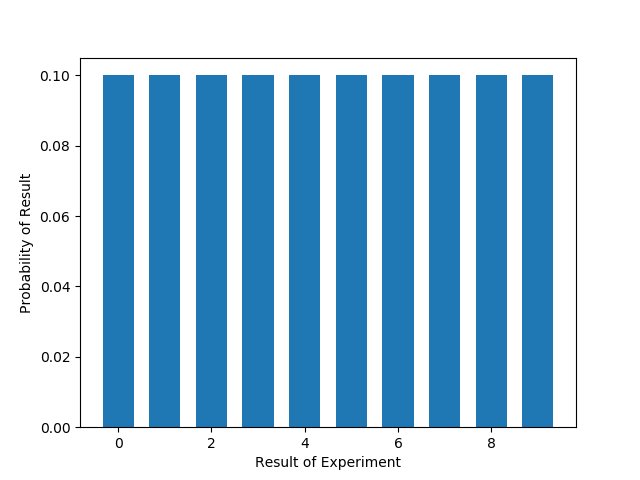
\includegraphics[width=0.75\textwidth]{img/uniform.png}\\
\caption{A discrete uniform probability distribution for an arbitrary experiment with 10 possible outcomes.}
\label{figure:uniform_distribution}
\end{figure}

\begin{definition}
A \emph{random bit} $b$ is a special case of a random number, such that the equiprobable sample space is $\Omega = \{0, 1\}$ \cite[s. 1.1.1]{rukhin2001statistical}.
\end{definition}

\begin{definition}
A \emph{random sequence} $s = (x_0, x_1, ..., x_n)$, as defined by Barker et al, is a sequence of random values $x_i$ resulting from $n$ independent selections. In other words, a random sequence consists of random numbers such that the probability distribution for any particular selection is entirely unaffected by previous selections. The random sequence has the same probability of being sampled as all other sequences of the same length \cite[p. 7]{barker2007recommendation} \cite[s. 1.1.1]{rukhin2001statistical}.
\end{definition}

Every binary sequence represents, in some encoding scheme, a unique numerical value. For example, the binary sequence $101$ is the unsigned integer representation of the number $5$. Thus there is an equivalence between random binary sequences and random numbers, in that the probability of randomly sampling any particular binary sequence of length $l$ from the set $\{0, 1\}$ is the same as that of selecting the number the sequence represents from the set of $2^l$ numbers that can be encoded with $l$ bits. As observed by Menezes et al, we can therefore regard the task of producing a random number as equivalent to the task of producing a random binary sequence \cite[p. 170]{menezes1996handbook}.

A key property of random numbers and random sequences is \emph{unpredictability}, for a sequence of random numbers, the probability of correctly guessing any value in the sequence is no greater than random chance \cite[p. 7]{barker2007recommendation}. The degree of unpredictability of a number sequence is quantified by the concept of \emph{entropy}, defined by Ferguson et al \cite[p. 12-13]{cover2012elements} as follows:

\begin{definition}
Let $X$ be a discrete random variable over a sample space $\Omega$ with a probability distribution function $p(x)=\mathbb{P}\{X=x\}, x\in\Omega$.  The entropy $H(X)$, measured in bits, of the discrete random variable $X$ is defined as
\begin{gather}\label{eq:entropy}
H(X) = -\sum_{x\in\Omega} p(x) \lg p(x)
\end{gather}
\end{definition}

According to Ferguson et al., entropy is a subjective quantity, in the sense that it depends on the amount of knowledge available about a value of interest. The entropy of an arbitrary number is different for an observer that knows the number, and for one that only knows the value is one of $2^{n}$ possible values. The concept is not explored in depth in this report, where it is mentioned, it will suffice to informally understand that the more uncertain we are about a sequence, the higher its entropy \cite[p. 137]{ferguson2010cryptography}.



\subsection{Random Number Generators}
In order to obtain sequences of random numbers for use in applications such as those mentioned above, \emph{random number generators} are used.

\begin{definition}
Menezes et al. define a random number generator as a software or hardware system that outputs random number (or bit) sequences. Key components of such a system are the \emph{entropy source}, which gives rise to the randomness in the output, and the \emph{entropy distillation} process, which is an algorithmic procedure applied to the produced values to improve the quality of the output sequence \cite{menezes1996handbook}.
\end{definition}

According to Ferguson et al and Menezes et al, entropy sources are commonly implemented in software, hardware, or both. Examples of entropy sources that are harnessed by software means include the timings of keystrokes on a computer user's keyboard, the current value of the system clock, the content of an I/O buffer, or any other measurable quantity in a computer system that is believed to exhibit random behavior. This conjecture does not always hold; for example, the time elapsed between keystrokes may not be accurately described by a uniform distribution, as an experienced typist may manage to keep their typing rate remarkably constant (with fluctuations on the order of several milliseconds). Care has to be taken to not overestimate the amount of entropy that can be derived from a source \cite[p. 138-139]{ferguson2010cryptography} \cite[p. 171-172]{menezes1996handbook}.

Ferguson et al and Menezes et al also discuss hardware entropy sources. These rely on physical processes that behave randomly. Commonly cited examples are emission times of particles during radioactive decay or thermal noise in a resistor. While there are very many such processes (in particular in the ``quantum realm" \cite{bierhorst2018experimentally}), physically based entropy sources are not guaranteed to be flawless. Even if a process behaves randomly, the outputs may nonetheless be biased or correlated, possibly due to manipulation by a third party. Furthermore, a third party may be able to observe the physical entropy source; while still random, the outputs would no longer have any entropy from the their perspective \cite[p. 138-139]{ferguson2010cryptography} \cite[p. 172]{menezes1996handbook}.

According to Ferguson, Schneier, and Kohno, there are several problems related to the practical use of truly random numbers. Real random data may not always be available, and even if available it is nonetheless always limited in quantity. For example, for an RNG relying on a user's keystrokes, it may be the case that the user has not been typing sufficiently. Waiting for more real random data to be acquired in order to receive random numbers is not a viable option for a number of applications \cite[p. 139]{ferguson2010cryptography}. Furthermore, as discussed above, it is difficult to ascertain how much entropy one is really getting from the source, not to mention that the source, in particular if implemented in hardware, may fail unexpectedly and become predictable \cite{ferguson2010cryptography}.



\subsection{Pseudo-Random Number Generators}\label{subsection:prngs}
A solution to many of the problems inherent to the use of truly random number generators is to use a \emph{pseudo-random number generator} \cite[p. 140]{ferguson2010cryptography}.

\begin{definition}
A pseudo-random number generator (PRNG) is a deterministic algorithm with an internal state $S_i$ \cite[p. 2]{kelsey1998cryptanalytic} which processes an input value $s$, known as the \emph{seed}, to produce a number sequence that may not tractably be distinguished from a truly random sequence by statistical means \cite[p. 170]{menezes1996handbook}. The current internal state and seed uniquely determine the PRNG's output (figure \ref{figure:prng_high_level}) \cite[p. 2]{kelsey1998cryptanalytic} \cite[s 1.1.4]{rukhin2001statistical}.

Following from the above, this investigation defines a PRNG as an implementation of a function $prng(s) : \mathbb{R} \rightarrow \mathbb{R}^n$, where $n$ is the length of the output sequence produced by the PRNG for some seed $s$. Alternatively, we can view each individual number in the output sequence as the product of some function $prng(s, S_i) : X \rightarrow \mathbb{R}$, where $X$ is the set of all tuples $(s, S_i)$.
\end{definition}

Implementations of PRNGs range in complexity and efficacy from simple \emph{linear congruential generators} \cite[p. 170]{menezes1996handbook} to the more complex \emph{Mersenne twister} \cite{matsumoto1998mersenne}. The concepts behind their operation are not considered in this report. Note that the internal state of the PRNG may be arbitrarily complex. For example, the \emph{ANSI X9.17 generator}, described by Menezes et al., takes further input parameters in addition to the random seed \cite[p. 173]{menezes1996handbook}. This investigation takes the view that any such additional inputs, provided they are not random and thus do not constitute a source of entropy for the generator, can be seen as a component of the internal state.

With the limitations of truly random number generators in mind, according to Menezes at al. the purpose of a PRNG is to ``take a small truly random sequence and expand it to a sequence of much larger length", in such a way that the output sequence fulfills some application-dependent randomness requirements \cite[p. 170]{menezes1996handbook}. In the context of security, the minimum requirement is that the length $l$ of the seed be such that it is unfeasible to carry out exhaustive search over all possible seeds. Randomness requirements for cryptographic use are considered in more detail in subsection \ref{subsection:crypto_requirements}.

\begin{figure}
\centering
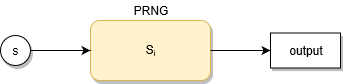
\includegraphics[width=0.6\textwidth]{img/conceptual_prng.png}\\
\caption{A high-level view of the operation of a PRNG \cite{kelsey1998cryptanalytic}.}
\label{figure:prng_high_level}
\end{figure}



\section{Random Numbers and Cryptography}
Random numbers are ubiquitous in computing, with applications in \emph{simulation}, \emph{sampling}, \emph{numerical analysis}, \emph{randomized algorithms}, \emph{decision making}, \emph{aesthetics}, and \emph{games} \cite[p. 1-2]{donald1998art}. Perhaps most importantly, random numbers are widely used in cryptography to secure communications \cite[p. 137]{ferguson2010cryptography}.

The notion of randomness is crucial in cryptography, because the security guarantees of systems such as encryption and decryption algorithms often rely on an adversary not knowing the value of some internal parameter \cite[p. 169]{menezes1996handbook} \cite[p. 1]{kelsey1998cryptanalytic}. It follows that the adversary should not have a good chance of being able to guess said parameters \cite[p. 2]{kelsey1998cryptanalytic}, meaning that their values should be unpredictable.


\subsection{Cryptographic Applications of Random Numbers}
As stated earlier, pseudo-random numbers are widely applied to cryptosystems, for example in encryption and decryption algorithms \cite[p. 169]{menezes1996handbook}. For example, the \emph{RSA (Rivest-Shamir-Adleman) algorithm}, as explained by Anderson \cite{anderson2010security}, is the canonical algorithm for performing public-key encryption and digital signatures. The RSA algorithm relies on two randomly chosen large prime numbers $p$ and $q$, which act as the private keys used by the two communicating parties. As these values must be kept secret from any third parties, they need to be selected randomly in such a manner than an attacker cannot predict them \cite[p. 171]{anderson2010security}.


\subsection{Cryptographically Secure Pseudo-Random Number Generators}\label{subsection:crypto_requirements}
As the outputs of a PRNG should be practically indistinguishable from truly random sequences, the basis for determining whether a PRNG is suitable for use in cryptographic applications is subjecting its outputs to a number of statistical tests \cite[p. 170]{menezes1996handbook}. From Menezes et al. and Rukhin et al. we obtain the following definitions, formulated in terms of statistical tests.

\begin{definition}
A \emph{statistical test} is a test which seeks to determine whether a sequences possesses some statistical property which is expected of a truly random sequence \cite[p. 175]{menezes1996handbook}. A statistical test computes a specific \emph{statistic} on the sample under evaluation \cite[p. 179]{menezes1996handbook}. Since the properties of a truly random sequence are known a priori and can be formulated in probabilistic terms, it is possible to determine the probability of the computed statistic appearing under the assumption of randomness \cite[s 1-3]{rukhin2001statistical}.
\end{definition}

\begin{definition}
A \emph{polynomial-time statistical test} is a test with a time complexity upper bound $O(l^k)$, where $l$ is the length of the sequence being tested and $k$ is a constant \cite[p. 171]{menezes1996handbook}.
\end{definition}

\begin{definition}
A PRNG passes the \emph{next-bit test} if no polynomial-time algorithm can predict the bit at position $n + 1$ in the output given the first $n$ bits with probability significantly greater than 0.5. Furthermore, a PRNG passes the next-bit test if, and only if, it passes all polynomial-time statistical tests \cite[p. 171]{menezes1996handbook}.
\end{definition}

\begin{definition}
A \textit{cryptographically secure pseudo-random number generator} (CSPRNG) is a pseudo-random number generator that passes the next-bit test \cite[p. 171]{menezes1996handbook}.
\end{definition}

Note that for real-world CSPRNGs, as with cryptosystems in general, security relies on the conjectured intractability of some underlying numerical problem \cite[p. 185]{menezes1996handbook}. As an example, the RSA algorithm relies on the computational complexity of the integer factorization problem \cite[p. 170-173]{anderson2010security}. This theoretical aspect of security is beyond the scope of this investigation and is not considered.



\subsection{Testing Number Sequences for Randomness}\label{subsection:testing_prngs}
Rukhin at al. point out that the degree of randomness of a number sequence can be evaluated by means of statical hypothesis testing \cite[s. 1-3]{rukhin2001statistical}.

\begin{definition}
According to Menezes et al., a \emph{statistical hypothesis} is ``an assertion about a distribution of one or more random variables", while a \emph{test} is ``a procedure [...] which leads to the acceptance or rejection of the hypothesis" \cite[p. 179]{menezes1996handbook}. The probability of incorrectly rejecting a statistical hypothesis is known as the \emph{significance level} $\alpha$ of the test \cite[p. 179]{menezes1996handbook}.
\end{definition}

Rukhin et al explain that, in testing number sequences for randomness, statistical tests are formulated to test the \emph{null hypothesis} $H_0$ that the sequence is random. Under the assumption of randomness, any statistical metric has a theoretical reference distribution \cite[p. 1.3]{rukhin2001statistical}. For this distribution, a \emph{critical value} is determined, which acts as a threshold; if the observed value exceeds the critical value, we reject the null hypothesis. We consider a value above the critical value to be so unlikely to occur under the assumption of randomness, that we can reasonably (though not certainly) reject the randomness hypothesis \cite[p. 1.3]{rukhin2001statistical} (figure \ref{figure:distribution}).

\begin{figure}
    \centering
    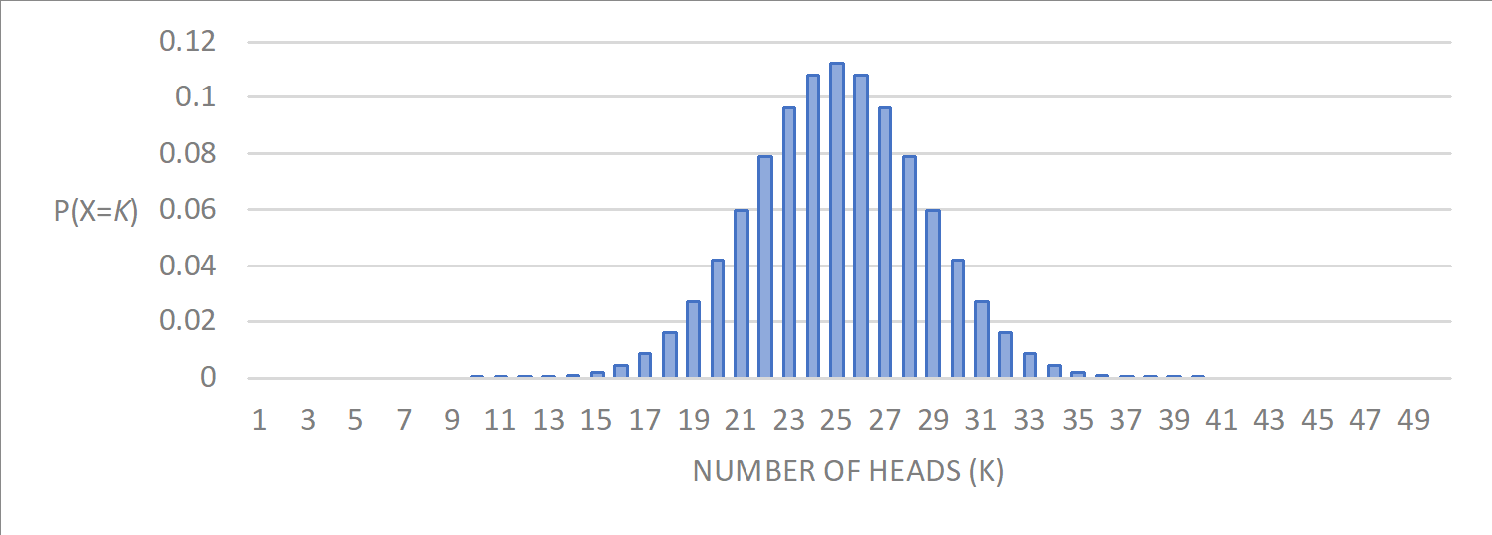
\includegraphics[width=1\textwidth]{img/distribution.png}\\
    \caption{The probability distribution of a random variable representing the number of 1s in a truly random binary sequence of length 50. Values at the tails of the distribution, such as 2 and 48, could be chosen as critical values; farther results are so unlikely that, upon observing them, one could justifiably question whether the sequence really is random}
    \label{figure:distribution}
\end{figure}

A simple example of a statistical randomness test, as explained by Menezes et al., is the \emph{frequency test}, which determines the number of 1s and 0s in the sequence. For a truly random sequence, as the length of the sequence tends to infinity the ratio of the two values approaches 1. That is, we expect the two values to be approximately the same \cite[p. 181]{menezes1996handbook}.

The NIST Test Suite is the accepted standard for testing random and pseudo-random bit generators \cite{lavasani2009practical}. It consists of a battery of statistical tests performed on files containing large binary sequences (on the order of $10^6$ bits with standard settings). Each test in the suite either accepts or rejects the null hypothesis \cite{rukhin2001statistical}. The NIST suite was found to be used throughout the majority of reviewed papers on PRNGs, and is accordingly used in this investigation.




\section{Artificial Neural Networks}
This section provides an introduction to neural networks, covering basic concepts such as the functioning of individual neurons in a network, how a neural network's parameters are updated to enable learning, and some common network topologies.


\subsection{Introduction to Neural Networks}\label{subsection:neural_intro}
\begin{definition}
According to Russel and Norvig, an \emph{artificial neural network} is a directed graph composed of \emph{units} or \emph{neurons} connected by directed \emph{links}. Each unit computes an arbitrary function $g$, called the \emph{activation function}, over a weighted sum of the unit's inputs. A link from unit $i$ to a unit $j$ carries the output of $i$'s activation function to $j$. Each such link has an associated \emph{weight} parameter $w_{ij}$, which is a coefficient applied to the activation value \cite[p. 727-731]{russel2009artificial}. Russel and Norvig define the function represented by a neuron $j$ as
\begin{gather}\label{eq:activation}
a_j = g(in_j) = g\left(\sum_{i=0}^{n} w_{ij}a_i\right)
\end{gather}
where $a_j$ is the neuron's output, $g$ is the neuron's activation function, and $j$ has $n$ input neurons $i$ with outputs $a_i$ and weights $w_{ij}$ \cite[p. 728]{russel2009artificial}.
\end{definition}

This can also be formulated in vector form as the inner product of inputs $\bm{a}_i$ and input weights $\bm{w}_{ij}$:
\begin{gather}\label{eq:activation_vector}
a_j = g(\bm{w}_{ij}\cdot\bm{a}_i)
\end{gather}

\begin{figure}
\centering
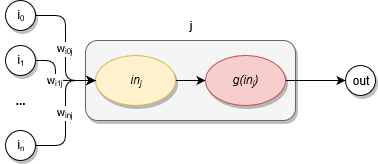
\includegraphics[width=0.6\textwidth]{img/neuron.png}\\
\caption{Schematic of the computation performed by a unit, drawn in accordance to the definitions given by Russel and Norvig \cite[p.728]{russel2009artificial}. A weighted sum $in_j$ of the unit's inputs is computed, and the resulting value becomes the argument of the activation function $g$. The activation's output is the node's output. This schematic corresponds to equation \ref{eq:activation}.}
\label{figure:neural_unit}
\end{figure}

A neural network as a whole, as explained by Russel and Norvig, computes a highly non-linear vector function $\bm{f}_{\bm{w}}(\bm{x})$ parameterized by its weights $\bm{w}$ \cite[p. 731, 732]{russel2009artificial}. The function $\bm{f}$ is the composition of $i$ functions $\bm{f}^{(i)}$ \cite[p. 164]{goodfellow2016deep}, which can be expressed as
 \begin{gather}\label{eq:neural_net_composition}
 \bm{f_w}(\bm{x}) = \bm{f}_{\bm{w}_{i-1}}^{(i-1)} (\bm{f}_{\bm{w}_{i-2}}^{(i-2)} ( \ldots \bm{f}_{\bm{w}_{0}}^{(0)}(\bm{x})))
\end{gather}
where $\bm{w_i}$ is the output weight vector for the units computing the function $\bm{f_{w_i}}^{(i)}$ \cite{goodfellow2016deep}.

According to Russel and Norvig, \emph{a neural network of sufficient size can represent any continuous function to an arbitrary degree of accuracy}, and, under certain conditions, can even represent discontinuous functions. However, difficulties arise in determining, for any particular network architecture, the set of functions it can represent \cite[p. 732]{russel2009artificial}. The particular properties of the network are determined by the topology and behavior of its units, which form the basis for the naming and categorization of networks \cite[p. 729]{russel2009artificial}. \todo{explain hyperparameter optimization}
\todo{mention recurrent networks}


\subsection{Learning in Neural Networks}
\begin{definition}
\emph{Training} an artificial neural network is an optimization problem which entails searching for a combination parameters $\bm{w}$ which results in the network approximating the desired function $f(x)$ as closely as possible \cite[p. 718]{russel2009artificial}. The most important related concepts are \emph{loss functions}, \emph{gradient descent}, and \emph{backpropagation}. todo{epoch and learning rate}
\end{definition}

\begin{definition}
Russel and Norvig define loss as ``the amount of utility lost" by the network producing $f_{pred}(x) = y'$ as its output when the correct output on an input $x$ is $f_{true}(x) = y$. A neural network's loss function $L(y, y')$ computes the loss for an output $y'$ and its corresponding correct output $y'$ \cite{russel2009artificial}. Intuitively, a loss function provides a quantitative assessment of how closely the neural network approximates the desired function (a good model will have low loss). The objective of learning is to find the parameters which minimize the loss function \cite[Linear classification: Support Vector Machine, Softmax]{karpathy2017cs231n}.
\end{definition}

\begin{definition}
Gradient descent is a numerical optimization algorithm used to train neural networks, in which the parameters of the network are iteratively updated into the direction opposite to the loss function's first-order gradient (computed with respect to the parameters) \cite[Optimization: Stochastic Gradient Descent]{karpathy2017cs231n}. Gradient descent is ubiquitous in the optimization of neural network loss functions. A high-level expression of gradient descent, from \cite{karpathy2017cs231n}, is as follows:

\begin{minted}{html}
  while True:
    weights_grad = evaluate_gradient(loss_fun, data, weights)
    weights += - step_size * weights_grad  # parameter update
\end{minted}
\end{definition}

An important design choice, according to Karpathy, is the number of inputs over which the loss is computed in order to perform a single update to the network's parameters. In \emph{batch gradient descent}, the loss is computed as an average of the loss for each input in the entire training dataset; in \emph{mini-batch gradient descent} the dataset is split into subsets, and a single parameter update is performed using each subset \cite[Optimization: Stochastic Gradient Descent]{karpathy2017cs231n}. In general, the larger the batch size, the more ``stable" the loss function is over training iterations, as the impact of single network inputs is diminished \cite[Neural Networks Part 3: Learning and Evaluation]{karpathy2017cs231n}. \todo{image of stable vs wiggly loss}

\begin{definition}
Lastly, backpropagation is an efficient algorithm for computing the partial derivative of a function of many variables by repeated application of the chain rule of derivation \cite[Backpropagation, Intuitions]{karpathy2017cs231n}. It is crucial as it enables efficient computation of the gradient of the loss function with respect to each parameter in the neural network \cite[Backpropagation, Intuitions]{karpathy2017cs231n}. Backpropagation is a core component of all modern machine learning software libraries.
\end{definition}

These three components enable learning in neural networks: the loss function quantifies the quality of the current parameters, gradient descent is the general optimization algorithm for modifying the parameters, and backpropagation enables efficient computation of gradients, making gradient descent on large networks practically feasible \cite[Optimization: Stochastic Gradient Descent]{karpathy2017cs231n}.



\subsection{Activation Functions}
The concept of an \emph{activation function} was briefly introduced in \ref{subsection:neural_intro}, as an arbitrary scalar function applied to the weighted sum of a unit's inputs to produce the unit's output. There are a number of standard activation functions that are commonly used \cite[Neural Networks Part 1: Setting up the Architecture]{karpathy2017cs231n}, of which two are considered here.

\begin{definition}
The \emph{rectified linear unit} activation, or ReLU, is an activation function $ReLU(x) : \mathbb{R} \rightarrow \mathbb{R}^{+}$ with the following expression form:
\begin{gather}\label{eq:relu}
ReLU(x) = max(0, x)
\end{gather}
\end{definition}.

The ReLU activation function works well in practice on a large number of problems \cite[Neural Networks Part 1: Setting up the Architecture]{karpathy2017cs231n}. However, it is possible for a ReLU unit to have its weights updated in a way that causes them to never be updated again, due to the 0 gradient for all negative inputs \cite[Neural Networks Part 1: Setting up the Architecture]{karpathy2017cs231n}. 

\begin{definition}
The \emph{leaky ReLU} function is an activation function $LReLU(x) : \mathbb{R} \rightarrow \mathbb{R}$ with the following expression form:
\begin{gather}\label{eq:leakyrelu}
LeakyReLU(x) = 
\begin{cases}
    x 							 & \text{if } x\geq 0\\
    \alpha{x}             & \text{otherwise}
\end{cases}
\end{gather}
where $\alpha$ is a (small) non-zero constant. For negative inputs close to 0, the outputs of the leaky ReLU are approximately equal to the outputs of ReLU. However, a leaky ReLU unit does not have a zero-gradient for any input, and thus cannot reach a state in which it stops updating, the way a ReLU unit would\cite[Neural Networks Part 1: Setting up the Architecture]{karpathy2017cs231n}.
\end{definition}

\begin{figure}
\centering
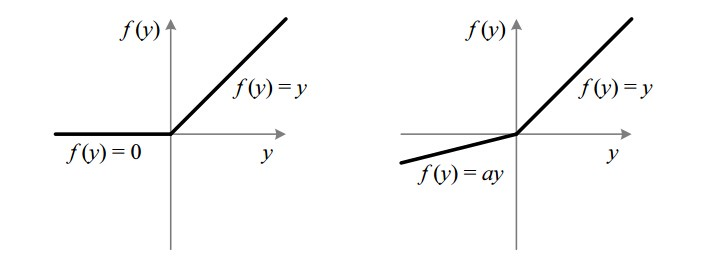
\includegraphics[width=0.7\textwidth]{img/relu.jpg}\\
\caption{Left: the ReLU function. Right: the LeakyReLU function. Note the zero gradient for negative inputs on the left, and how this problem is adressed on the right. Image courtesy of \cite{sharma2017activation}.}
\label{figure:relu}
\end{figure}



\subsection{Fully Connected Feed-Forward Networks}
\begin{definition}
The simplest form of deep neural network is called a \emph{fully connected feed-forward neural network}, or \emph{multilayer perceptron}. A fully connected feed-forward (FCFF) network is a directed acyclic graph in which information strictly flows from the network's input units towards its output units \cite[p. 164]{goodfellow2016deep}. Feed-forward networks are typically arranged into fully connected \emph{layers} of units, where the number of layers is called the \emph{depth} of the network; the first layer is the \emph{input layer}, followed by a number of \emph{hidden layers} and finally the \emph{output layer} \cite[p. 164-165]{goodfellow2016deep}. The number of units in the largest layer is referred to as the \emph{width} of the network (figure \ref{figure:feedforward}) \cite[p. 164-165]{goodfellow2016deep}.
\end{definition}

The number of units in the input and output layers are bound by the dimensionality of the input data and the dimensionality of the expected outputs. In a fully connected feed-forward network, the operation of each layer can be characterized as a simple matrix operation, whereby a layer's output vector is matrix multiplied with the layer's output weight matrix, and then passed to the next layer where the activation function is applied \cite[p. 170-171]{goodfellow2016deep}. It follows that the network as a whole is a sequence of matrix multiplications and element-wise applications of non-linearity.

\begin{figure}
\centering
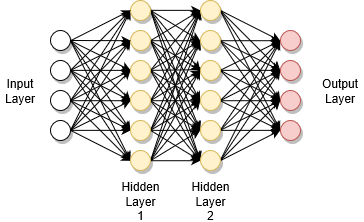
\includegraphics[width=0.65\textwidth]{img/feedforward_nn.png}\\
\caption{Simple example of the structure of a feedforward network. The network has two hidden layers, for a total depth of 4. The network's width is 6, as given by the size of the hidden layers. Image drawn using draw.io \cite{jgraph2018draw}}
\label{figure:feedforward}
\end{figure}



\subsection{Convolutional Neural Networks}
\begin{definition}
A \emph{convolutional neural network} is a more specialized neural network architecture characterized by the fact that at least one pair of layers is connected in such a manner as to perform a \textit{convolution} rather than a general matrix multiplication \cite[p. 326]{goodfellow2016deep}.
\end{definition}

\begin{definition}
According to Karpathy \cite{karpathy2017cs231n}, a \emph{convolutional layer} is a collection of units further subdivided into equally sized groups referred to as \emph{filters}. Each unit in a filter receives inputs from $k$ consecutive units in the previous layer, where $k$ is referred to as the \emph{kernel size} or \emph{receptive field} of the convolutional layer. The \emph{stride} $s$ of the layer determines the sparsity of the units in each filter (figure \ref{figure:convolution1d}). A convolutional layer may have multiple filters, each with the same connection topology to the previous layer. The number of filters is referred to as the \emph{depth} of the layer, while the dimensions of each individual filter are referred to as the \emph{width} and \emph{height} of the layer \cite[Convolutional Neural Networks: Architectures, Convolution / Pooling Layers]{karpathy2017cs231n}.
\end{definition}

All units in a filter share the same input weights (an optimization called \emph{parameter sharing}). Thus every unit in the filter computes the same function on a specific subset of the previous layer's outputs. Intuitively, the filter as a whole ``looks for'' specific instances of some pattern in the input; a stack of $n$ filters looks for instances of $n$ different patterns (figure \ref{figure:convolution1d}) \cite[Convolutional Neural Networks: Architectures, Convolution / Pooling Layers]{karpathy2017cs231n}.

Karpathy explains that the dimensionality of a convolutional layer's output is $d + 1$, where $d$ is the dimensionality of the output of the previous layer: with $N$ filters, the convolutional layer outputs $N$ matrices with the same dimensionality as the layer's input. Because of this, convolutional layers are usually followed by \emph{pooling layers}, which are non-parametric layers that down-sample the convolutional layer's outputs \cite[Convolutional Neural Networks: Architectures, Convolution / Pooling Layers]{karpathy2017cs231n}. This expansion along the depth-dimension, followed by down-sampling in the width and height dimensions, is shown in figure \ref{figure:conv_pooling}.

\begin{figure}
    \centering
    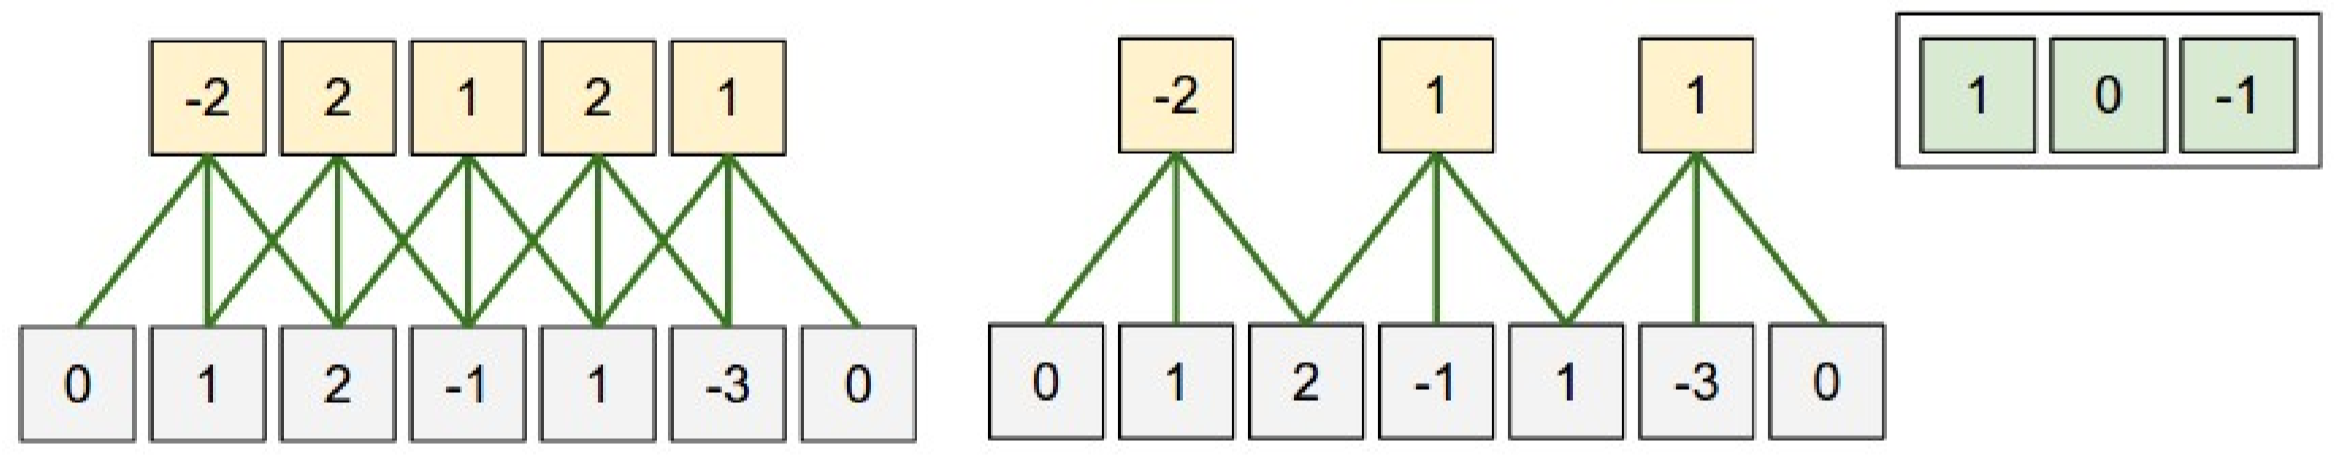
\includegraphics[width=0.85\textwidth]{img/convolution.png}\\
    \caption{A representation of the connectivity between the units of a 1-dimensional input layer (white) and the filters in a convolutional layer (yellow), with each convolutional unit's input weights shown in the squares. In both images, the kernel size is 3; on the left the stride of the layer is 1, while on the right it is 2. Furthermore, the convolutional layer on the left has two filters. Note how both filters are connected to the input in the same way, and how each filter has its own set of input weights. The image is based on the CS231n lecture notes by Andrej Karpathy \cite[Convolutional Neural Networks: Architectures, Convolution / Pooling Layers]{karpathy2017cs231n} and was drawn with draw.io \cite{jgraph2018draw}.}
    \label{figure:convolution1d}
\end{figure}

\begin{figure}
\centering
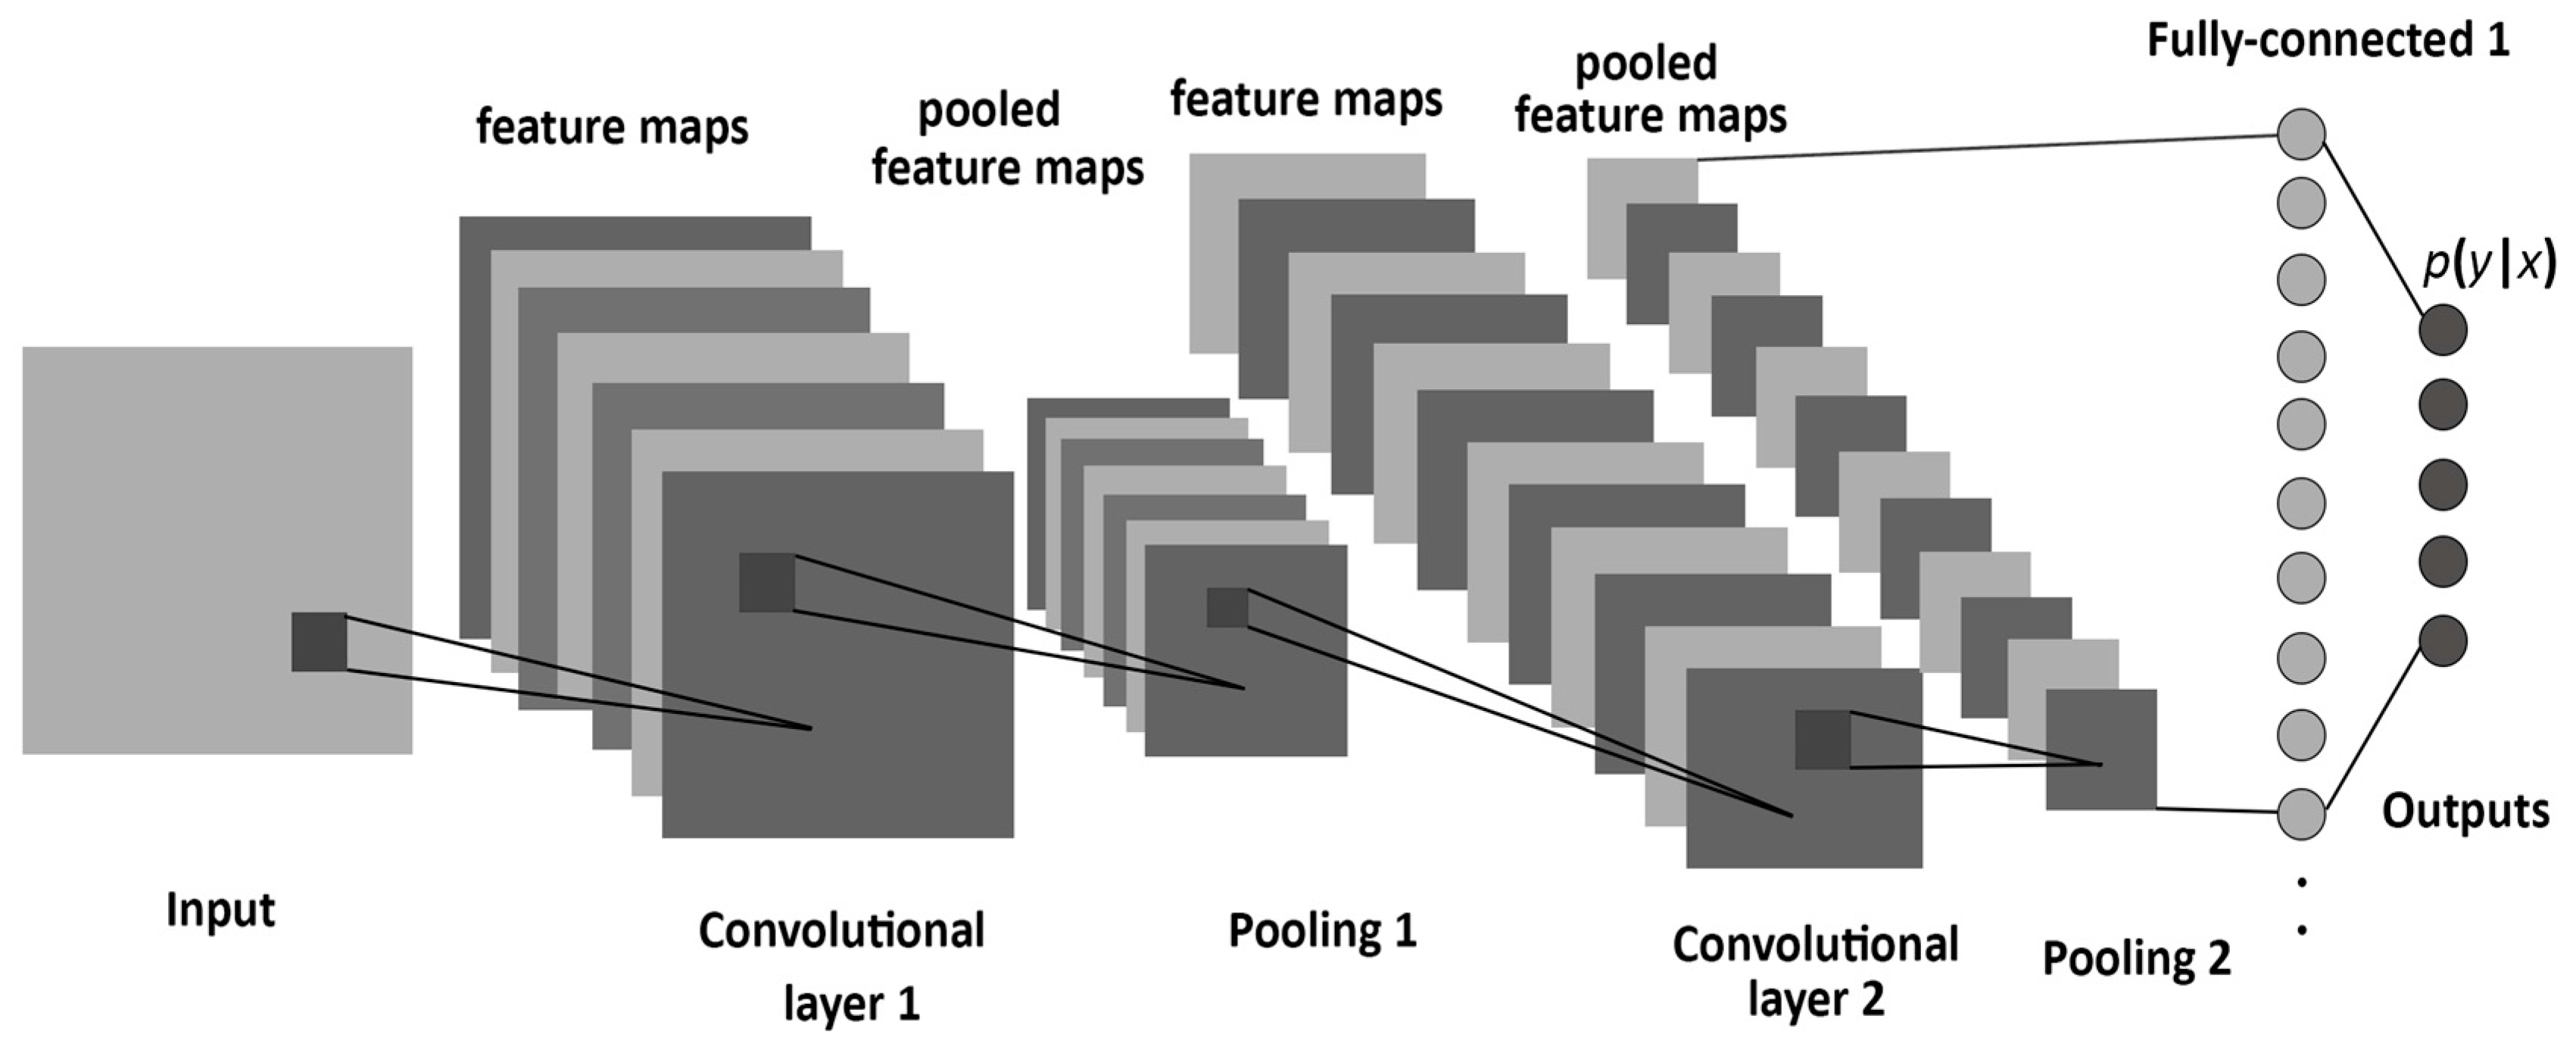
\includegraphics[width=1\textwidth]{img/conv_pooling.png}\\
\caption{A convolutional layer preserves the dimensions of its input matrix, but produces an output with a larger depth dimensions depending on the number of filters. This is followed by pooling layers, which down-sample the data in the width and height dimensions. Image courtesy of \cite{albelwi2017framework}.}
\label{figure:conv_pooling}
\end{figure}



\subsection{Generative Adversarial Networks}\label{subsection:generativeadversarial}
Machine learning models may be classified as being either \textit{discriminative} or \textit{generative}. An example of discriminative models is neural networks that map images to content labels \cite[p. 1]{goodfellow2014generative}. Generative models, on the other hand, learn to mimic the training set. Goodfellow et al introduced \emph{generative adversarial networks} (GANs) in 2014, succinctly defining them as a ``framework for estimating generative models via an adversarial process", where a discriminative model is used to train a generative model by scrutinizing its outputs \cite[p. 1]{goodfellow2014generative}.

\begin{definition}
Let $Z$ be a random variable with any distribution, and let $T$ be a random variable representing a dataset with a probability distribution $p_{data}$. A \emph{generative model} learns a mapping $gen(z) : Z \rightarrow M$, where $M$ is a random variable with a distribution $p_{model}$ that approximates $p_{data}$ \cite{goodfellow2016nips.}
\end{definition}

\begin{definition}
Let $Z$ be a random variable with any distribution, and let $T$ be a random variable representing a dataset with a probability distribution $p_{data}$. A generative adversarial network (GAN) consists of two artificial neural networks, a \emph{generator} $G$ and a \emph{discriminator} $D$. The generator represents a function $G_{\theta_{g}}(\bm{z}) : Z \rightarrow M$ parameterized by weights $\theta_g$, which maps inputs $\bm{z} \in Z$ to an output $\bm{x}$ in $M ~ p_{model}$. The discriminator represents a function $D_{\theta_d}(\bm{x}) : T \cap M \rightarrow \mathbb{R}$ that outputs a scalar representing the probability that $\bm{x}$ was sampled from $T$ rather than produced by the generator (figure \ref{figure:gan}).

The discriminator is trained to maximize the probability of assigning the correct label to inputs sampled from $T$ and generated by $G$. In turn, the generator is trained to minimize $\log{1 - D(G(\bm{z}))}$. Goodfellow et all \cite[p. 3]{goodfellow2014generative} showed that this is equivalent to saying that, during training, $D$ and $G$ engage in a two-player minimax game with value function $V(G, D)$, formulated as follows:
\begin{gather}\label{eq:gan_train}
\min_G{\max_D{V(G, D)}} = \mathbb{E}_{\bm{x}~p_{data}(\bm{x})}[\log{D(\bm{x})}] + \mathbb{E}_{\bm{z}~p_{\bm{z}}(\bm{z})}[\log{1 - D(G(\bm{z}))}]
\end{gather}
\end{definition}

A mini-batch stochastic gradient descent training algorithm for a GAN, as given by Goodfellow et al but slightly simplified, is shown below.
\begin{minted}{html}
    for i in range(training_iterations):
      for k in range(steps):
        sample mini-batch from data distribution
        sample mini-batch from generator
        update discriminator by gradient descent
      sample mini-batch of noise from noise distribution
      update generator by gradient descent
\end{minted}
Goodfellow et all also showed that, provided $G$ and $D$ have sufficient capacity, and at each step of the above algorithm $D$ is allowed to reach its optimum given the current $G$, then $p_{model}$ converges to $p_{data}$ \cite[p. 5]{goodfellow2014generative}.

\begin{figure}
    \centering
    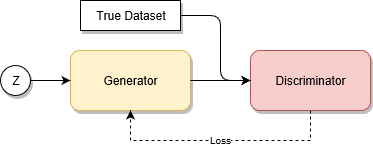
\includegraphics[width=0.6\textwidth]{img/gan.png}\\
    \caption{The conceptual structure of a generative adversarial network. The outputs of the generator are fed into the discriminator along with samples from the original dataset; the performance of the discriminator is factored into the loss function of the generator. Image drawn with draw.io \cite{jgraph2018draw}.}
    \label{figure:gan}
\end{figure}



\section{Related Work}\label{section:related_work}
Literature review found that few efforts have been made to train neural networks to act as pseudo-random number generators. In this section, the findings of some key relevant papers are reviewed.



\subsection{Papers on Using Neural Networks as Pseudo-Random Number Generators}
Overall, the literature review carried out for this investigation showed that little research has been carried out on the implementation of PRNGs using neural networks. A small number of such papers was identified, but all were relatively obscure, possibly due to reliance on complex neural network architectures and contrived training procedures in an attempt to encourage chaotic behavior \cite{desai2011pseudo} \cite{desai2012pseudo} \cite{tirdad2010hopfield} \cite{wen2014exponential}.

For example, a 2012 paper by Veena Desai et al from the Gogte Institute of Technology, \textit{Pseudo random number generator using time delay neural network}, failed to produce a viable neural network-based PRNG, and identified the computational complexity of training networks with thousands of neurons as one of the key challenges \cite{desai2012pseudo}.

Other publications include Desai's earlier 2011 paper \textit{Pseudo random number generator using Elman neural network}, as well as the 2010 paper \textit{Hopfield Neural Networks as Pseudo-Random Number Generators} by Tirdad and Sadeghian. In both cases the conclusions were mixed. Desai's paper reported ``satisfactory results'' on a subset of the performed statistical tests, with unexplained particularly poor performance on one of the tests \cite{desai2011pseudo}. Tirdad and Sadeghian achieved a strong performance on the NIST test suite in some of the reported experiments \cite{tirdad2010hopfield}. However, the opinion of the author of this report is that their implementation is contrived and exceedingly complex. \todo{more detail because this is interesting}


\subsection{Learning to Protect Communications with Adversarial Neural Cryptography}
The 2016 paper by Google Brain researches Martin Abadi and David Andersen investigates the ability of neural networks to learn some form of symmetric-key encryption scheme in a multiagent environment, enabling some agents to communicate securely. The paper's abstract states:

\say{We ask whether neural networks can learn to use secret keys to protect information from other neural networks. Specifically, we focus on ensuring confidentiality properties in a multiagent system, and we specify those properties in terms of an adversary. Thus, a system may consist of neural networks named Alice and Bob, and we aim to limit what a third neural network named Eve learns from eavesdropping on the communication between Alice and Bob. We do not prescribe specific cryptographic algorithms to these neural networks; instead, we train end-to-end, adversarially. We demonstrate that the neural networks can learn how to perform forms of encryption and decryption, and also how to apply these operations selectively in order to meet confidentiality goals.} \cite{abadi2016learning}

The paper's conclusion mentions pseudo-random number generation as a possible avenue of further investigation, providing the original inspiration behind this work.





%----------------------------------------------------------
% DESIGN AND IMPLEMENTATION
%----------------------------------------------------------
\chapter{Design and Implementation}\label{chapter:design}
This section provides an in-depth explanation of the conceptual design of the system and how it relates to the research hypothesis, the technologies used to implement it, and the details of the implementation.



\section{Conceptual Design}\label{section:conceptual_design}
As stated, the aim of this investigation is to determine whether it is possible to train a neural network to output pseudo-random number sequences. Previous work has attempted to answer this question by using recurrent architectures to encourage chaotic behavior (see section \ref{section:related_work}). In contrast, this investigation takes a more intuitive approach, conjecturing that a simple fully-connected feed-forward network of sufficient size can learn a function whose inputs appear random.

For simplicity, we view a pseudo-random number generator as a system implementing some function
\begin{gather}\label{eq:conceptual_prng}
prng(s) : \mathbb{R} \rightarrow \mathbb{R}^n
\end{gather}
where $s$ is a truly random seed value, $n$ is a very large value, and the outputs of $prng$ fulfill a set of criteria for randomness. In regards to each individual output value, we can characterize a PRNG as a function 
\begin{gather}
prng(s, S_i) : X \rightarrow \mathbb{R}
\end{gather}
where $S_i$ is the current state of the generator, and $X$ is the set of all tuples $(s, S_i)$. That is, a PRNG is fundamentally a function which maps a single seed value to a very large (unique) output sequence, such each element of the sequence is determined by the generator's state. A generator neural network, $G$, should learn a function which approximates $prng$.

We can abstract the complexity of the internal state of PRNGs by using a stateless neural network, and equivalently representing the generator's ``state" as a component of the network's input instead. This conceptual difference is demonstrated in figure \ref{figure:conceptual_difference}. Thus the neural network should learn a function
\begin{gather}
G_{\theta_{G}}(s, o_t) : \mathbb{R}^i \rightarrow \mathbb{R}^n
\end{gather}
where $s$ is a truly random seed value, $o_t$ model's a PRNG's internal state and can be seen as an ``offset" into the full output sequence for $s$, and $i$ is the dimensionality of the network input.

\begin{figure}
\centering
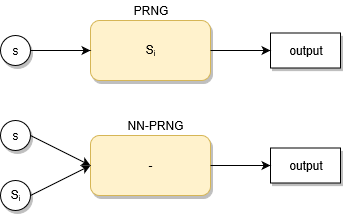
\includegraphics[width=0.5\textwidth]{img/conceptual_design.png}\\
\caption{The conceptual difference in the common implementation of PRNGs (top) and the implementation using GANs in this work (bottom). Image produced using draw.io \cite{jgraph2018draw}.}
\label{figure:conceptual_difference}
\end{figure}

This work views the generation of pseudo-random numbers in a cryptographic setting as a fundamentally adversarial task: the goal of good CSPRNG design is to minimize the probability of an intelligent adversary correctly guessing future outputs. This is analogous to the generative adversarial network framework, where a discriminator attempts to find patterns in the generator's output, and the generator minimizes its probability of doing so correctly. Thus it is natural to formulate the task of generating pseudo-random number sequences using a GAN. Two distinct approaches are considered, termed the \textit{discriminative approach} and the \textit{predictive approach}, respectively (figure \ref{figure:approach_comparison}). 

In the discriminative approach, the adversary is a standard discriminator network, which receives number sequences as inputs both from the generator and a source of true randomness, and outputs the probability that a sequence is truly random. The input sequences are labeled as truly random or not random, and the discriminator is trained to better discern the two classes. In order to prevent the discriminator from performing better than it would by making random guesses, the generator has to learn to mimic the truly random sequences.

The predictive approach is loosely based on the idea of the theoretical next bit test, outlined in section \ref{subsection:crypto_requirements}. Each sequence of length $n$ produced by the generator is split, such that the first $n - 1$ values are passed to the adversary as input, and the $n$th value is used as the corresponding label; the predictor is trained to output the $n$th value in the generator's output sequence based on all previous values. Again, the generator's goal is to modify its behavior in order to minimize the probability of the predictor making a correct guess.

Both approaches are elegantly intuitive. The former is a direct application of the standard GAN framework, which requires the generator to learn the uniform probability distribution characteristic of truly random number sequences. The latter models closely the actual goals of a PRNG and its adversary in a cryptographic setting. Unlike previous work, this investigation follows an important guideline given by Russel and Norvig: \textit{``As a general rule, it is better to design performance measures according to what one actually wants in the environment, rather than according to how one thinks the agent should behave"} \cite[p. 37]{russel2009artificial}.

\begin{figure}
\centering
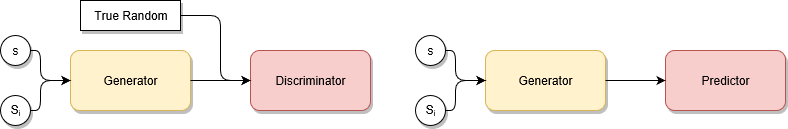
\includegraphics[width=0.99\textwidth]{img/approach_comparison.png}\\
\caption{The two approaches differ at the conceptual level in the the discriminative approach (left) requires a source of true randomness which it attempts to emulate, while the predictive approach (right) is an even purer ``game" between the two networks, with no side inputs. Image produced using draw.io \cite{jgraph2018draw}.}
\label{figure:approach_comparison}
\end{figure}



\subsection{Generative Model}
The generator is a fully connected feed-forward neural network implementing the function $G_{\theta_{G}}(s, o_t) : \mathbb{R}^2 \rightarrow \mathbb{R}^m$. It takes two input values, where the first is a truly random seed, and the second is a representation of the PRNG state; the output is a 1D real vector of length $m$. For any specific seed $s$, the complete pseudo-random sequence produced by the generator is given by the concatenation of all the output sequences $\forall o_t\ G_{\theta_{G}}(s, o_t)$, where $s$ is fixed.

The generator consists of five fully connected feed-forward layers (figure \ref{figure:architecture_generator}). The input layer, as well as the hidden layers, use the leaky ReLU activation function which is currently the general recommendation for generic application \cite[Neural Networks Part 1: Setting up the Architecture]{karpathy2017cs231n}. The output layer uses an activation function which computes a modulus operation on every element in the output vector, squeezing the values into a desired range. A popular variant of the stochastic gradient descent algorithm called Adam is used, which adaptively computes separate learning rates for each parameter \cite{kingma2014adam} \cite[Optimization: Stochastic Gradient Descent]{karpathy2017cs231n}.

Two slightly different variants of the generator are implemented, referred to as \mintinline{python}{jerry} and \mintinline{python}{janice}. The former uses a ``squared difference" loss function and is trained using the discriminative approach, while the latter uses an ``absolute difference" loss function and is trained using the predictive approach. The two implementations are identical otherwise.

\begin{figure}
\centering
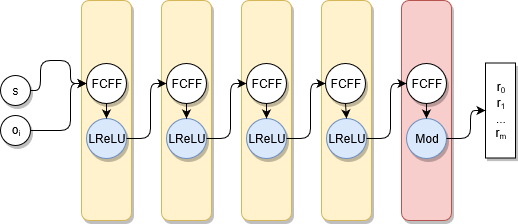
\includegraphics[width=0.7\textwidth]{img/generator.png}\\
\caption{Architecture of the generator. Each fully connected feed-forward layer's activation function (blue) is shown; the output layer (red) differs from the other layers in that it does not use the leaky ReLU activation, but rather a modulus function. Image produced using draw.io \cite{jgraph2018draw}.}
\label{figure:architecture_generator}
\end{figure}

\textbf{TODO: talk about the modulus activation}



\subsection{Discriminative Model}
The discriminator and the predictor are convolutional neural networks implementing the functions
\begin{gather}
disc(\bm{r}) : \mathbb{R}^m \rightarrow [0, 1] \\
pred(\bm{r}_{split}) : \mathbb{R}^{m - 1} \rightarrow \mathbb{R}
\end{gather}
respectively, where $\bm{r}$ is the generator's output vector, $\bm{r}_{split}$ is the output vector without the last element, and $m$ is the output vector's size. The discriminator takes as inputs sequences of length $m$ and outputs a scalar representing the probability the sequence is truly random. The predictor's inputs are sequences of length $m-1$ produced by the generator, using which the network attempts to guess the $m$th value in the sequence.

Apart from the input size and the meaning of the output, the discriminator and the predictor share the same architecture. The input first passes through four convolutional layers for 1-dimensional inputs.

\begin{figure}
\centering
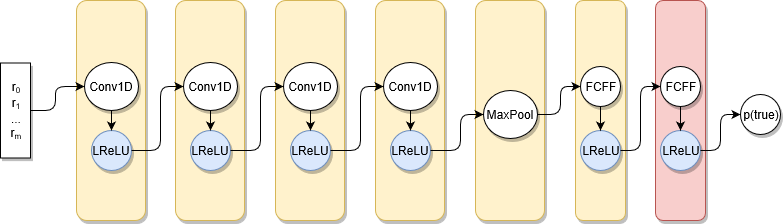
\includegraphics[width=1\textwidth]{img/discriminator.png}\\
\caption{Convolutional discriminator architecture. The output of the generator is convolved multiple times in order to extract higher-level features from the sequence; this is followed by pooling to reduce the output size, and fully connected feed-forward layers to produce the final classification output. Image produced using draw.io \cite{jgraph2018draw}.}
\label{figure:architecture_conv}
\end{figure}

\begin{figure}
\centering
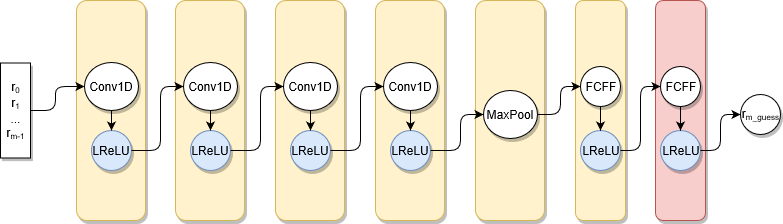
\includegraphics[width=1\textwidth]{img/predictor.png}\\
\caption{Convolutional predictor architecture. The design is shared with the discriminator, but the size of the input sequence and the meaning of the output scalar are different. The predictor produces a guess for the last value in the generator's output based on the previous values. Image produced using draw.io \cite{jgraph2018draw}.}
\label{figure:architecture_conv}
\end{figure}



\subsection{Predictive Model}



\section{Implementation Technologies}
The system was developed using version 3.6 of the Python programming language, which is popular in the machine learning field due to its conciseness and the large ecosystem of software libraries for numerical computing \cite{numpy}. In addition to NumPy, which is ubiquitous in numerical computation using Python \cite{numpy}, the main software librariy used for this project is TensorFlow. The latter is an ``open source library for numerical computation" released by Google, which is commonly used for machine learning \cite{tensorflow}. Most of the code in the implementation deals with abstractions defined in the TensorFlow API.

While Python and the TensorFlow library are popular in the machine learning community, alternatives abound. Programming languages considered for the project included Java and C++, both of which have popular deep learning libraries. Furthermore, TensorFlow is not the only machine learning library available for Python: options include Theano, PyTorch, CNTK, and scikit-learn.

Choosing a language, a software library, or a software framework for a particular task is not always straightforward. In this case, Python and TensorFlow were selected due to Python's legibility and simplicity, which supports rapid prototyping, as well as TensorFlow's popularity in the machine learning field, which ensures the availability of abundant documentation, tutorials, and more \cite{bhatia2017why}. The use of these particular technologies is not a critical aspect of this research.

\subsection{Introduction to TensorFlow}
An introductory guide to the central concepts and functionality of TensorFlow is provided on the software library's website \cite{tensorflow2018intro}. The TensorFlow version used in this project is 1.6.

The central concept is that of the \textit{tensor}, an $n$-dimensional generalization of vectors and matrices. Tensors have properties such as \textit{rank} and \textit{shape}, which specify the number of dimensions of a tensor as well as its size in each dimension \cite{tensorflow2018intro}. TensorFlow programs perform a series of operations on tensors.

At the highest level of abstraction, a TensorFlow program consists of a \textit{Computational Graph} and a \textit{Session}. The former is a directed graph consisting of tensor operations applied to a set of inputs, and defines the topology of a machine learning model. The operations specified in the graph are not computed by the Python interpreter, but rather are first compiled and then executed in TensorFlow's C++ runtime. The Python application interface to the runtime is defined by a TensorFlow Session \cite{tensorflow2018graphs}. When interacting with a session, the act of passing specific inputs to a model for a particular session is referred to as \textit{feeding}, while retrieving the value of a tensor in the graph at a particular time during execution is referred to as \textit{fetching} \cite{tensorflow2018intro}.

The package \mintinline{python}{tf.contrib.gan} in TensorFlow's Python API enables the programmer to easily define generative adversarial networks.



\subsection{Supporting Technologies}
Development and deployment required a mix of free as well as proprietary supporting tools. Most notable are the distributed software version control system \mintinline{python}{git} \cite{git2018}, and the popular containerization tool \mintinline{python}{Docker} \cite{docker2018} for deployment.

Software used also includes the Jetbrains PyCharm integrated development environment \cite{jetbrains2018pycharm}, and Microsoft's free code editor VSCode. Early tests of the implementation's performance were executed on virtual machines in Google's, Amazon's, and Digital Ocean's cloud services, with a mix of CPU-focused and GPU-focused instance types.

Training of the model was carried out on an HPC cluster, access to which was provided by the School of Electronic Engineering and Computer Science at Queen Mary University of London. The cluster consists of 5 machines, each with 64 CPU cores, 256 GB RAM, and no GPUs. The code was executed within a \mintinline{python}{Docker} container.


\section{Software Design}
This section outlines the structure of the software implementing the concepts from section \ref{section:conceptual_design}. The code broadly follows the examples provided in TensorFlow's tutorials \cite{tensorflow2018tutorials} \cite{tensorflow2018tfgan}. The structure of the implementation is as follows:

\begin{minted}{html}
    > adversarial-csprng    
        > src
            > components
                __init__.py
                activations.py
                operations.py
            > utils
                __init__.py
                debug.py
                decode_nist.py
                file_utils.py
                input.py
                operations.py
                visualize.py
            main.py
        .gitignore
        Dockerfile
        nist.sh
        readme.md
        requirements.txt
        transfer.sh
\end{minted}

The files in the root directory include a \mintinline{python}{.gitignore} specifying which files in the project should not be version-controlled by \mintinline{python}{git}, a \mintinline{python}{Dockerfile} specifying the build procedure for the Docker container used to run the system, a convenient \mintinline{python}{readme}, a \mintinline{python}{requirements} file listing the project's Python dependencies, and two shell scripts to automate the retrieval of evaluation results from a remote compute cluster.

The \mintinline{python}{src} package contains all Python software modules. At its root is the \mintinline{python}{main.py} module, which is the software's intended entry point and contains the implementation's core. The \mintinline{python}{components} package contains modules defining custom TensorFlow functions used as components of the TensorFlow computational graph. Lastly, the \mintinline{python}{utils} package contains a number of modules defining utility functions broadly categorized by functionality. These are not considered in the report, but are available in the supporting documentation.

The code is structured in a procedural manner (as opposed to object-oriented). The rationale for this design choice is based on a number of factors. Firstly, localizing all of the core logic into \mintinline{python}{main.py} improves flexibility in prototyping and experimenting: as most of the core logic is prone to frequent change, bundling it into a single module improves productivity by reducing the amount of time spent looking for particular implementation details. In other words, in a project such as this, \emph{low-level details matter at the high level}, and abstracting them into object-oriented modules is inconvenient. Furthermore, the procedural approach is the convention of the field. Following convention facilitates communication.



\subsection{System Parameterization}
Several aspects of the systems are parameterized to provide ease of modification in the prototyping phase. In some cases simple command-line arguments are also supported, simplifying the running of experiments with different training setups. 

The most imporant parameter specifiable via command-line arguments is \mintinline{python}{HPC_TRAIN}, which specifies whether the model is being trained on the HPC cluster or tested during development. In testing mode, the scale of the model and the duration of training are drastically reduced, allowing a rapid test of correct execution of the system. Other parameters specifiable via the command line are the networks' learning rate and the number of training iterations.

\begin{minted}[fontsize=\small]{python}
# main settings
# set to true when training on HPC to collect data
HPC_TRAIN = '-t' not in sys.argv
LEARN_LEVEL = 2 if '-highlr' in sys.argv else 0 if '-lowlr' in sys.argv else 1

# hyper-parameters
OUTPUT_SIZE = 8
MAX_VAL = 65535
OUTPUT_BITS = 16
BATCH_SIZE = 2046 if HPC_TRAIN else 10
LEARNING_RATE = {2: 0.1, 1: 0.02, 0: 0.008}[LEARN_LEVEL]
GEN_WIDTH = 30 if HPC_TRAIN else 10
DATA_TYPE = tf.float64

# training settings
TRAIN = ['-nodisc' not in sys.argv, '-nopred' not in sys.argv]
STEPS = 1000000 if '-long' in sys.argv else 150000 if HPC_TRAIN else 40
PRE_STEPS = 100 if HPC_TRAIN else 5
ADV_MULT = 3
\end{minted}


\subsection{Generative Model}
The generator $G$ has the same implementation for both the discriminative approach, where it is referred to as \mintinline{python}{jerry}, and the predictive approach, where it is referred to as \mintinline{python}{janice}. The model's architecture is defined in \mintinline{python}{main.py} using TensorFlow as follows:

\begin{minted}[fontsize=\small]{python}
input_layer = tf.reshape(noise, [-1, 2])
outputs = fully_connected(input_layer, GEN_WIDTH, activation=leaky_relu)
outputs = fully_connected(outputs, GEN_WIDTH, activation=leaky_relu)
outputs = fully_connected(outputs, GEN_WIDTH, activation=leaky_relu)
outputs = fully_connected(outputs, GEN_WIDTH, activation=leaky_relu)
outputs = fully_connected(outputs, OUTPUT_SIZE, activation=modulo(MAX_VAL))
return outputs
\end{minted}

\mintinline{python}{GEN_WIDTH} parameterizes the number of units in the hidden layers. The \mintinline{python}{reshape} operation is used to cast input tensors to an appropriate size. The second argument specifies the shape to which input tensors are cast, where the first value is the tensor's size in the \textit{batch dimension}, and any following values represent the dimensionality of the input samples. The batch dimension refers to the number of input samples in a single batch. In TensorFlow \mintinline{python}{-1} is a special flag signifying dynamic batch size, which allows the model to process its inputs in batches of any size, rather than a fixed size. The output layer's \mintinline{python}{modulo} activation function is detailed in subsection \ref{subsection:custom_ops}.


\subsection{Discriminative and Predictive Models}
The discriminator $D$, \mintinline{python}{diego}, and the predictor $P$, \mintinline{python}{priya}, share the same architecture with the exception of the width of the input layer (\mintinline{python}{OUTPUT_SIZE} for \mintinline{python}{diego}, \mintinline{python}{OUTPUT_SIZE - 1} for \mintinline{python}{priya}). This is explained in section \ref{section:conceptual_design}. The convolutional architecture of the adversaries is implemented in \mintinline{python}{main.py} as follows:

\begin{minted}[fontsize=\small]{python}
input_layer = tf.reshape(inputs, [-1, size])
outputs = tf.expand_dims(input_layer, 2)
outputs = conv1d(outputs, filters=4, kernel_size=2, strides=1, 
                 padding='same', activation=leaky_relu)
outputs = conv1d(outputs, filters=4, kernel_size=2, strides=1, 
                 padding='same', activation=leaky_relu)
outputs = conv1d(outputs, filters=4, kernel_size=2, strides=1, 
                 padding='same', activation=leaky_relu)
outputs = conv1d(outputs, filters=4, kernel_size=2, strides=1, 
                 padding='same', activation=leaky_relu)
outputs = max_pooling1d(outputs, pool_size=2, strides=1)
outputs = flatten(outputs)
outputs = fully_connected(outputs, 4, activation=leaky_relu)
outputs = fully_connected(outputs, 1, activation=leaky_relu)
return outputs
\end{minted}

The \mintinline{python}{flatten} and \mintinline{python}{reshape} operations are used to modify the shape of tensors in order to connect layers with different shapes. Unlike the generator, where a custom activation function is used in order to introduce greater non-linearity, all layers in the adversary models use the popular leaky rectified linear unit activation.



\subsection{Custom Tensor Operations}\label{subsection:custom_ops}
The \mintinline{python}{components} package contains modules implementing neural network functionality that is not a part of the TensorFlow API, including the custom activation function \mintinline{python}{modulo}.

\mintinline{python}{modulo(divisor, withActivation=None)} is a closure returning a custom tensor function that computes the element-wise modulus $\mod{divisor}$ of its input tensor. Using a closure allows the creation of a function object with the desired parameters, which can then be passed to the TensorFlow API. The \mintinline{python}{modulo} function can additionally wrap another activation function, though this feature is not used.


\subsection{Obtaining Training Data}
Input data for training and evaluating the networks is generated by functions defined in the \mintinline{python}{utils.input} module. This includes two functions for producing a training dataset which return equivalent data structures, with the difference that one returns it as a NumPy array and the other as a TensorFlow tensor. The module also defines a function that produces an input dataset as a NumPy array which is used to evaluate the models.

A training dataset is produced as follows (the NumPy version is identical in structure as the TensorFlow API and NumPy API share many design aspects):

\begin{minted}[fontsize=\small]{python}
def get_input_tensor(batch_size, max_val) -> tf.Tensor:
    return tf.transpose(
        tf.stack(
            [tf.fill([batch_size], tf.random_uniform(shape=[], minval=0, maxval=max_val)),
             tf.random_uniform(shape=[batch_size], minval=0, maxval=batch_size)],
        ))
\end{minted}

The evaluation dataset is generated as follows:

\begin{minted}[fontsize=\small]{python}
def get_eval_input_numpy(seed, length, batch_size) -> np.ndarray:
    data = []
    offset = 0

    for batch_num in range(length):
        batch = []
        for item in range(batch_size):
            batch.append([seed, offset])
            offset = offset + 1
        data.append(batch)

    return np.array(data)
\end{minted}

Documentation strings were removed for brevity.



\subsection{Defining and Training the Discriminative GAN}\label{subsection:training_disc}
The discriminative GAN is defined using TensorFlow's \mintinline{python}{tf.contrib.gan} package, which simplifies the implementation of a standard GAN consisting of a generator and discriminator. The GAN is structured as follows:

\begin{minted}[fontsize=\small]{python}
# build the GAN model
discgan = tfgan.gan_model(
    generator_fn=generator,
    discriminator_fn=adversary_conv(OUTPUT_SIZE),
    real_data=tf.random_uniform(shape=[BATCH_SIZE, OUTPUT_SIZE]),
    generator_inputs=input.get_input_tensor(BATCH_SIZE, MAX_VAL)
)

# Build the GAN loss.
discgan_loss = tfgan.gan_loss(
    discgan,
    generator_loss_fn=tfgan.losses.least_squares_generator_loss,
    discriminator_loss_fn=tfgan.losses.least_squares_discriminator_loss)

# Create the train ops, which calculate gradients and apply updates to weights.
train_ops = tfgan.gan_train_ops(
    discgan,
    discgan_loss,
    generator_optimizer=GEN_OPT,
    discriminator_optimizer=OPP_OPT)
\end{minted}

The core of the main training loop is as follows:

\begin{minted}[fontsize=\small]{python}
for step in range(STEPS):
    train_steps_fn(sess, train_ops, global_step, train_step_kwargs={})

    # if performed right number of steps, log
    if step % LOG_EVERY_N == 0:
        sess.run([])
        gen_l = discgan_loss.generator_loss.eval(session=sess)
        disc_l = discgan_loss.discriminator_loss.eval(session=sess)

        debug.print_step(step, gen_l, disc_l)
        losses_jerry.append(gen_l)
        losses_diego.append(disc_l)
\end{minted}

\subsection{Defining and Training for the Predictive GAN}\label{subsection:training_pred}
The predictive approach does not fit the standard GAN framework, and thus was not easily implementable with \mintinline{python}{tf.contrib.gan}. It was implemented using more general low-level TensorFlow functionality. The GAN is defined as follows:

\begin{minted}[fontsize=\small]{python}
# janice tensor graph
janice_input_t = tf.placeholder(shape=[BATCH_SIZE, 2], dtype=tf.float32)
janice_output_t = generator(janice_input_t)
janice_true_t = tf.strided_slice(janice_output_t, [0, -0], [BATCH_SIZE, 1], [1, 1])
priya_pred_t = tf.placeholder(shape=[BATCH_SIZE, 1], dtype=tf.float32)
# priya tensor graph
priya_input_t = tf.placeholder(shape=[BATCH_SIZE, OUTPUT_SIZE - 1], dtype=tf.float32)
priya_label_t = tf.placeholder(shape=[BATCH_SIZE, 1], dtype=tf.float32)
priya_output_t = adversary_conv(OUTPUT_SIZE - 1)(priya_input_t)

# losses and optimizers
priya_loss = tf.losses.absolute_difference(priya_label_t, priya_output_t)
janice_loss = -tf.losses.absolute_difference(janice_true_t, priya_pred_t)
janice_optimizer = GEN_OPT.minimize(janice_loss)
priya_optimizer = OPP_OPT.minimize(priya_loss)
\end{minted}

The main training loop is as follows:

\begin{minted}[fontsize=\small]{python}
for step in range(STEPS):
    batch_inputs = input.get_input_numpy(BATCH_SIZE, MAX_VAL)
    # generate
    janice_output_n = sess.run([janice_output_t],
                               feed_dict={janice_input_t: batch_inputs})
    priya_input_n, priya_label_n = operations.slice_gen_out(janice_output_n[0])
    # update priya
    priya_output_n = None
    priya_loss_epoch = None
    for adv in range(ADV_MULT):
        _, priya_loss_epoch, priya_output_n = sess.run([priya_optimizer, priya_loss, priya_output_t],
                                                       feed_dict={priya_input_t: priya_input_n,
                                                                  priya_label_t: priya_label_n})
    # update janice
    _, janice_loss_epoch = sess.run([janice_optimizer, janice_loss],
                                    feed_dict={priya_pred_t: priya_output_n,
                                               janice_input_t: batch_inputs})

    # log and evaluate
    if step % LOG_EVERY_N == 0:
        debug.print_step(step, janice_loss_epoch, priya_loss_epoch)
        losses_janice.append(janice_loss_epoch)
        losses_priya.append(priya_loss_epoch)
\end{minted}



%----------------------------------------------------------
% EXPERIMENTS
%----------------------------------------------------------
\chapter{Experiments}\label{chapter:experiments}
This section outlines the experimentation phase of the project, including the experimentation plan, the precise procedure followed, the experiment parameters, and the results obtained.


\section{Experimentation Plan}
The aim of the experiments is to determine quantitatively the extent to which training the implemented GANs improves the randomness properties of the generators' outputs. These are measured by producing large files of generator output values to be analyzed using the NIST statistical test suite, both before and after a generator is trained.

\textbf{Independent variable}: whether the generative adversarial network has been trained or not. In other words, the generator's weight parameters are the independent variable.

\textbf{Dependent variable}: the result produced by the NIST test suite on a file containing a large number sequence produced by the generator on a fixed input.

\textbf{Controlled variables}: the following variables are unchanged throughout the entire experimental procedure:
\begin{enumerate}
    \itemsep0em
    \item Contents of input dataset used to produce the sequences to be evaluated using NIST
    \item Number of training epochs for the GANs
    \item Number of adversary epochs per each generator epoch
    \item Architecture of the generator
    \item Architecture of the discriminator
    \item Architecture of the predictor
    \item Learning rate of the networks
    \item Range of output values
    \item Mini-batch size used in processing inputs
\end{enumerate}

In summary, in each experiment, the randomness properties of the generator's outputs are assessed before and after training; the only changed quantity is the network's paramaters that have been optimized during training.


\section{Experimental Procedure}
The precise procedure for each experiment is as follows:

\begin{enumerate}
    \itemsep0em
    \item Start the system on the HPC machine.
    \item Create the pre-defined and unchanging evaluation dataset.
    \item Generate output number sequences by giving evaluation dataset as input to generator.
    \begin{enumerate}
        \itemsep0em
        \item Compute output vector for each input vector.
        \item Round real numbers to nearest integer. If the outputs are randomly distributed over a range $[a,b]$ where $a,b \in \mathbb{R}^+$, then they will also be randomly distributed over the range $[a,b]$ where $a,b \in \mathbb{Z}^+$.
        \item Store integers as hex strings in a text file prefixed with 0\_. Hex is used to reduce the number of characters in the file.
    \end{enumerate}
    \item Train the generative adversarial network. The generator and the adversary are trained in turn, with the adversary performing multiple parameter updates for each update made by the generator.
    \item Generate output number sequences by giving evaluation dataset as input to generator.
    \begin{enumerate}
        \itemsep0em
        \item Compute output vector for each input vector.
        \item Round real numbers to nearest integer. If the outputs are randomly distributed over a range $[a,b]$ where $a,b \in \mathbb{R}^+$, then they will also be randomly distributed over the range $[a,b]$ where $a,b \in \mathbb{Z}^+$.
        \item Store integers as hex strings in a text file prefixed with 1\_. Hex is used to reduce the number of characters in the file.
    \end{enumerate}
    \item Retrieve files containing generated number sequences using \mintinline{python}{scp}.
    \item Convert the text file's contents from hex characters to binary characters using the \mintinline{python}{decode_nist.py} utility.
    \item Run the NIST test suite on the converted file, performing all tests with default/recommended settings.
    \item Store the testing result files produced by the NIST test suite.
\end{enumerate}

For both approaches 10 experiments are carried out. In each experiment the GAN is trained for 200000 epochs, with the adversary being trained 3 times at each epoch (see subsection \ref{subsection:generativeadversarial} for the rationale behind this choice). 

Training is performed with mini-batches of 2046 data points, while the learning rate of the networks is set to 0.02. Both values were manually selected during prototyping as they resulted in good performance. The generator outputs real numbers constrained to the range $[0, 2^{16}-1]$, which are rounded to the nearest integer and converted to unsigned 16-bit integers for evaluation. The evaluation dataset consists of 400 batches of 2046 inputs, for a total of 818400 input samples. The generator produces 8 real numbers for each input, and each real number yields 16 bits for the output sequence. In total, each evaluation output consists of 104755200 bits. 

The NIST test suite is applied with the recommended setting of using 1000000 bits for each test. The test suite includes 188 separate tests, referred to from here onward as a \emph{test}, each repeated 10 times. Each repetition will be referred to as a \emph{test instance}. For each test, NIST reports the number of individual instances that passed, as well as a p-value for the distribution of p-values of the 10 test instances. A test can fail in one of two ways: either the number of passed instances is insufficient, or the p-value for the p-value distribution is below a critical value. See appendix \ref{appendix:sample} for a sample of the test suite's output.


\section{Results}
The statistical test results from the 20 training instances are collated here. Tables \ref{table:before_training} and \ref{table:after_training} show the performance of the generator neural networks before and after training. Table \ref{table:after_training_avg} shows the average performance after training for the two approaches, while table \ref{table:training_change} shows, for each experiment, the change in performance resulting from training. Lastly, table \ref{table:avg_result} shows the average improvement for the discriminative and predictive approaches, across all 10 experiments.

The symbols in the tables have the following meanings: $i$ identifies the experiment, with $D_i$ and $P_i$ referring to discriminative and predictive experiments, respectivey. $T$ refers to the overall number of separate tests carried out by the NIST test suite, while $T_I$ refers to the number of total test instances. $F_I$ and $F_{I\%}$ refers to the number of failed test instances and the percentage of failed test instances, respectively. $F_p$ represents the number of tests failed due to an abnormal distribution of the p-values of the underlying test instances. $F_T$ and $F_{\%}$ refer to the absolute number and percentage of separate tests failed, respectively. In tables \ref{table:after_training_avg}, ref{table:training_change} and \ref{table:avg_result}, the convention followed is that $\Delta$ refers to the change in some quantity, and the angle brackets $\langle \rangle$ refer to tge average value of the enclosed quantity.  

\begin{table}[H]
    \begin{tabularx}{\textwidth}{lXXXXXXX} \toprule
    {$i$}     & {$T$} 	& {$T_I$}	& {$F_I$} 	& {$F_{I\%} / \%$}		& {$F_p$} 	& {$F_T$} 	& {$F_{\%} / \%$} \\ \midrule
    $D_1$  & 188   	& 1802		& 1800	 	    & 99.9				& 188	 	& 188	 	& 100 \\
    $D_2$  & 188   	& 1802 		& 1791  		& 99.4				& 188	 	& 188	 	& 100 \\
    $D_3$  & 188  	& 1802 		& 1798  		& 99.8				& 188	 	& 188	 	& 100 \\
    $D_4$  & 188   	& 1802 		& 1802  		& 100.0			    & 188  		& 188  		& 100 \\
    $D_5$  & 188   	& 1802 		& 1788   		& 99.2				& 188  		& 188  		& 100 \\
    $D_6$  & 188  	& 1802 		& 1792  		& 99.4				& 188  		& 188 		& 100 \\
    $D_7$  & 188   	& 1802 		& 1799  		& 99.8				& 188  		& 188  		& 100 \\
    $D_8$  & 188   	& 1802 		& 1801  		& 99.9				& 188  		& 188  		& 100 \\
    $D_9$  & 188   	& 1802 		& 1802  		& 100.0			    & 188  		& 188  		& 100 \\
    $D_{10}$ & 188  & 1802 		& 1791  		& 99.4				& 188  		& 188  		& 100 \\ \midrule
    $P_1$  & 188   	& 1802 		& 1789    	    & 99.3				& 188  		& 188  		& 100 \\
    $P_2$  & 188   	& 1802 		& 1802  		& 100.0			    & 188  		& 188  		& 100 \\
    $P_3$  & 188   	& 1802 		& 1799  		& 99.8				& 188  		& 188  		& 100 \\
    $P_4$  & 188   	& 1802 		& 1802  		& 100.0			    & 188  		& 188  		& 100 \\
    $P_5$  & 188   	& 1802 		& 1792   		& 99.4				& 188  		& 188  		& 100 \\
    $P_6$  & 188   	& 1802 		& 1798  		& 99.8				& 188  		& 188  		& 100 \\
    $P_7$  & 188   	& 1802 		& 1792  		& 99.4				& 188  		& 188  		& 100 \\
    $P_8$  & 188   	& 1802 		& 1801  		& 99.9				& 188  		& 188  		& 100 \\
    $P_9$  & 188   	& 1802 		& 1802  		& 100.0			    & 188  		& 188  		& 100 \\
    $P_{10}$ & 188  & 1802 		& 1801  		& 99.9				& 188  		& 188  		& 100 \\ \bottomrule
\end{tabularx}
\caption[Test results for untrained generators]{Test results for untrained generators.}
\label{table:before_training}
\end{table}


\begin{table}[H]
    \begin{tabularx}{\textwidth}{lXXXXXXX} \toprule
    {$i$}  & {$T$} 	& {$T_I$}	& {$F_I$}   	& {$F_{I\%} / \%$}		    & {$F_p$} 	    & {$F_T$} 	    & {$F_{\%} / \%$} \\ \midrule
    $D_1$  & 188   	& 1802		& 29    	 	& 1.6				    & 3  	 		& 3  	 		& 2 \\
    $D_2$  & 188   	& 1724 		& 109  		    & 6.3					& 5  	 		& 11	 		& 6 \\
    $D_3$  & 188  	& 1724 		& 123  		    & 7.1   				& 4  	 		& 11	 		& 6 \\
    $D_4$  & 188   	& 1828 		& 168  		    & 9.2   				& 9      		& 18    		& 10 \\
    $D_5$  & 188   	& 1854 		& 49   			& 2.7					& 3  		    & 5		  		& 3 \\
    $D_6$  & 188  	& 1776 		& 30	  		& 1.7					& 5		  		& 5	 			& 3 \\
    $D_7$  & 188   	& 1854 		& 21	  		& 1.1					& 4		  		& 4		  		& 2 \\
    $D_8$  & 188   	& 1776 		& 46	  		& 2.6					& 5		 		& 5		  		& 3 \\
    $D_9$  & 188   	& 1802 		& 25	  		& 1.4					& 3		 		& 3	 			& 2\\
    $D_{10}$ & 188  & 1854 		& 14	  		& 0.8					& 2		 		& 4		 		& 2 \\ \midrule
    $P_1$  & 188   	& 1802 		& 39		 	& 2.2					& 2 			& 4		 		& 2 \\
    $P_2$  & 188   	& 1828 		& 27	  		& 1.5					& 3		 		& 3		 		& 2 \\
    $P_3$  & 188   	& 1828 		& 35	  		& 1.9					& 3		 		& 4		 		& 2 \\
    $P_4$  & 188   	& 1828 		& 100  		    & 5.5					& 2		 		& 8		  		& 4 \\
    $P_5$  & 188   	& 1802 		& 52	   		& 2.9					& 2		 		& 3		 		& 2 \\
    $P_6$  & 188   	& 1880 		& 111  		    & 5.9					& 4		 		& 9		 		& 5 \\
    $P_7$  & 188   	& 1802 		& 25	  		& 1.4					& 3		 		& 3		 		& 2 \\
    $P_8$  & 188   	& 1880 		& 96	  		& 5.1					& 2		 		& 4		  		& 2 \\
    $P_9$  & 188   	& 1854 		& 36	  		& 1.9					& 2		 		& 3 			& 2 \\
    $P_{10}$ & 188  & 1802 		& 37  			& 2.1					& 4		 		& 4		 		& 2 \\ \bottomrule
\end{tabularx}
\caption[Test results for trained generators]{Test results for trained generators.}
\label{table:after_training}
\end{table}


\begin{table}[H]
    \begin{tabularx}{\textwidth}{lXXXXXXX} \toprule
    {$i$}   & {$T$} 	& {$\langle T_I \rangle$}	& {$\langle F_I \rangle$}   	& {$\langle F_{I\%} \rangle / \%$}		    & {$\langle F_p \rangle$} 	    & {$\langle F_T \rangle$} 	    & {$\langle F_{\%} \rangle / \%$} \\ \midrule
    $D$     & 188  & 1800 		& 61	  		& 3.5					& 4.3		 		& 6.9		 		& 3.9 \\ \midrule
    $P$     & 188  & 1830 		& 56  			& 3.0					& 2.7		 		& 4.5		 		& 2.5 \\ \bottomrule
\end{tabularx}
\caption[Average test results for trained generators]{Average test results for trained generators.}
\label{table:after_training_avg}
\end{table}


\begin{table}[H]
    \begin{tabularx}{\textwidth}{lXXXX} \toprule
    {$i$}  & {$\Delta F_{I\%} / \%$}	            & {$\Delta F_p$} 	    & {$\Delta F_T$} 	        & {$\Delta F_{\%} / \%$} \\ \midrule
    $D_1$  & -98.3 							& -185 					& -185    	 				& -98 \\
    $D_2$  & -93.1 							& -183 					& -177  					& -94 \\
    $D_3$  & -92.7							& -184 					& -177  					& -94 \\
    $D_4$  & -90.8 							& -179 					& -160 					    & -90 \\
    $D_5$  & -96.5 							& -185 					& -183						& -97 \\
    $D_6$  & -97.7 							& -183 					& -183	  					& -97 \\
    $D_7$  & -98.7 							& -184 					& -184	  					& -98 \\
    $D_8$  & -97.3 							& -183 					& -183	  					& -97 \\
    $D_9$  & -98.6 							& -185 					& -185	  					& -98 \\
    $D_{10}$ & -98.6 						& -186 					& -184	  					& -98 \\ \midrule
    $P_1$  & -97.1  						& -186 					& -184		 				& -98 \\
    $P_2$  & -98.5  						& -185 					& -185	  					& -98 \\
    $P_3$  & -97.9 							& -185 					& -184	  					& -98 \\
    $P_4$  & -94.5  						& -186 					& -180  					& -96 \\
    $P_5$  & -96.5 							& -186 					& -187	   					& -98 \\
    $P_6$  & -93.9  						& -184 					& -179  					& -95 \\
    $P_7$  & -98.0  						& -185 					& -185	  					& -98 \\
    $P_8$  & -94.8  						& -186 					& -184	  					& -98 \\
    $P_9$  & -98.1  						& -186 					& -185	  					& -98 \\
    $P_{10}$ & -97.8  						& -184 					& -184						& -98 \\ \bottomrule
\end{tabularx}
\caption[Result improvement from before to after training]{Improvements in the measured quantities as a result of training the networks.}
\label{table:training_change}
\end{table}


\begin{table}[H]
    \begin{tabularx}{\textwidth}{lXXXX} \toprule
    {$i$}     & {$\langle \Delta F_{I\%} \rangle / \%$}	& {$\langle \Delta F_p \rangle$} 	& {$\langle \Delta F_T \rangle$} 	& {$\langle \Delta F_{\%} \rangle / \%$} \\ \midrule
    $D$ & -96.2 						& -183.7					& 	-180.1	  					& -96.1 \\ \midrule
    $P$ & -96.7  						& -185.3					& -183.6						& -97.5 \\ \bottomrule
\end{tabularx}
\caption[Average performance change across all experiments]{Average performance change for the discriminative and predictive approaches across all tests.}
\label{table:avg_result}
\end{table}


\section{Evaluation}\label{subsection:evaluation}
The results show that, prior to training, the parameters of the function represented by the generator network are not suitable for the production of pseudo-random numbers. As seen in table \ref{table:before_training}, the generator's outputs fail to pass any tests, with a 100\% rate of failure in every experiment. A visualization of the generator's outputs before training (figures \ref{figure:visualize_discriminative_before} and \ref{figure:visualize_predictive_before}) shows that the output of the network follows extremely predictable patterns.

As seen in table \ref{table:after_training}, both the discriminatively and predictively trained generators show very strong performance on the test suite, consistently achieving below 10\% failure rate in all but one experiment. Furthermore, the vast majority of experiments resulted in a failure rate below 5\%. As seen in figures \ref{figure:visualize_discriminative_after} and \ref{figure:visualize_predictive_after}, the patternicity of the generator's output is no longer visible.

Table \ref{table:training_change} more legibly quantifies the change in performance achieved in each experiment. In most experiments the absolute change in failure percentage points was greater than 95\%. 

Table \ref{table:avg_result} averages the values for the discriminative and predictive approaches across the 10 experiments performed. On average, the predictive approach performed slightly better in terms of passed test instances. A more noticeable 
- on average predictive approach had slightly larger improvements

- loss landscape looks weird af

\begin{figure}
    \centering
    \textbf{Output Sample, Before Discriminative Training}
    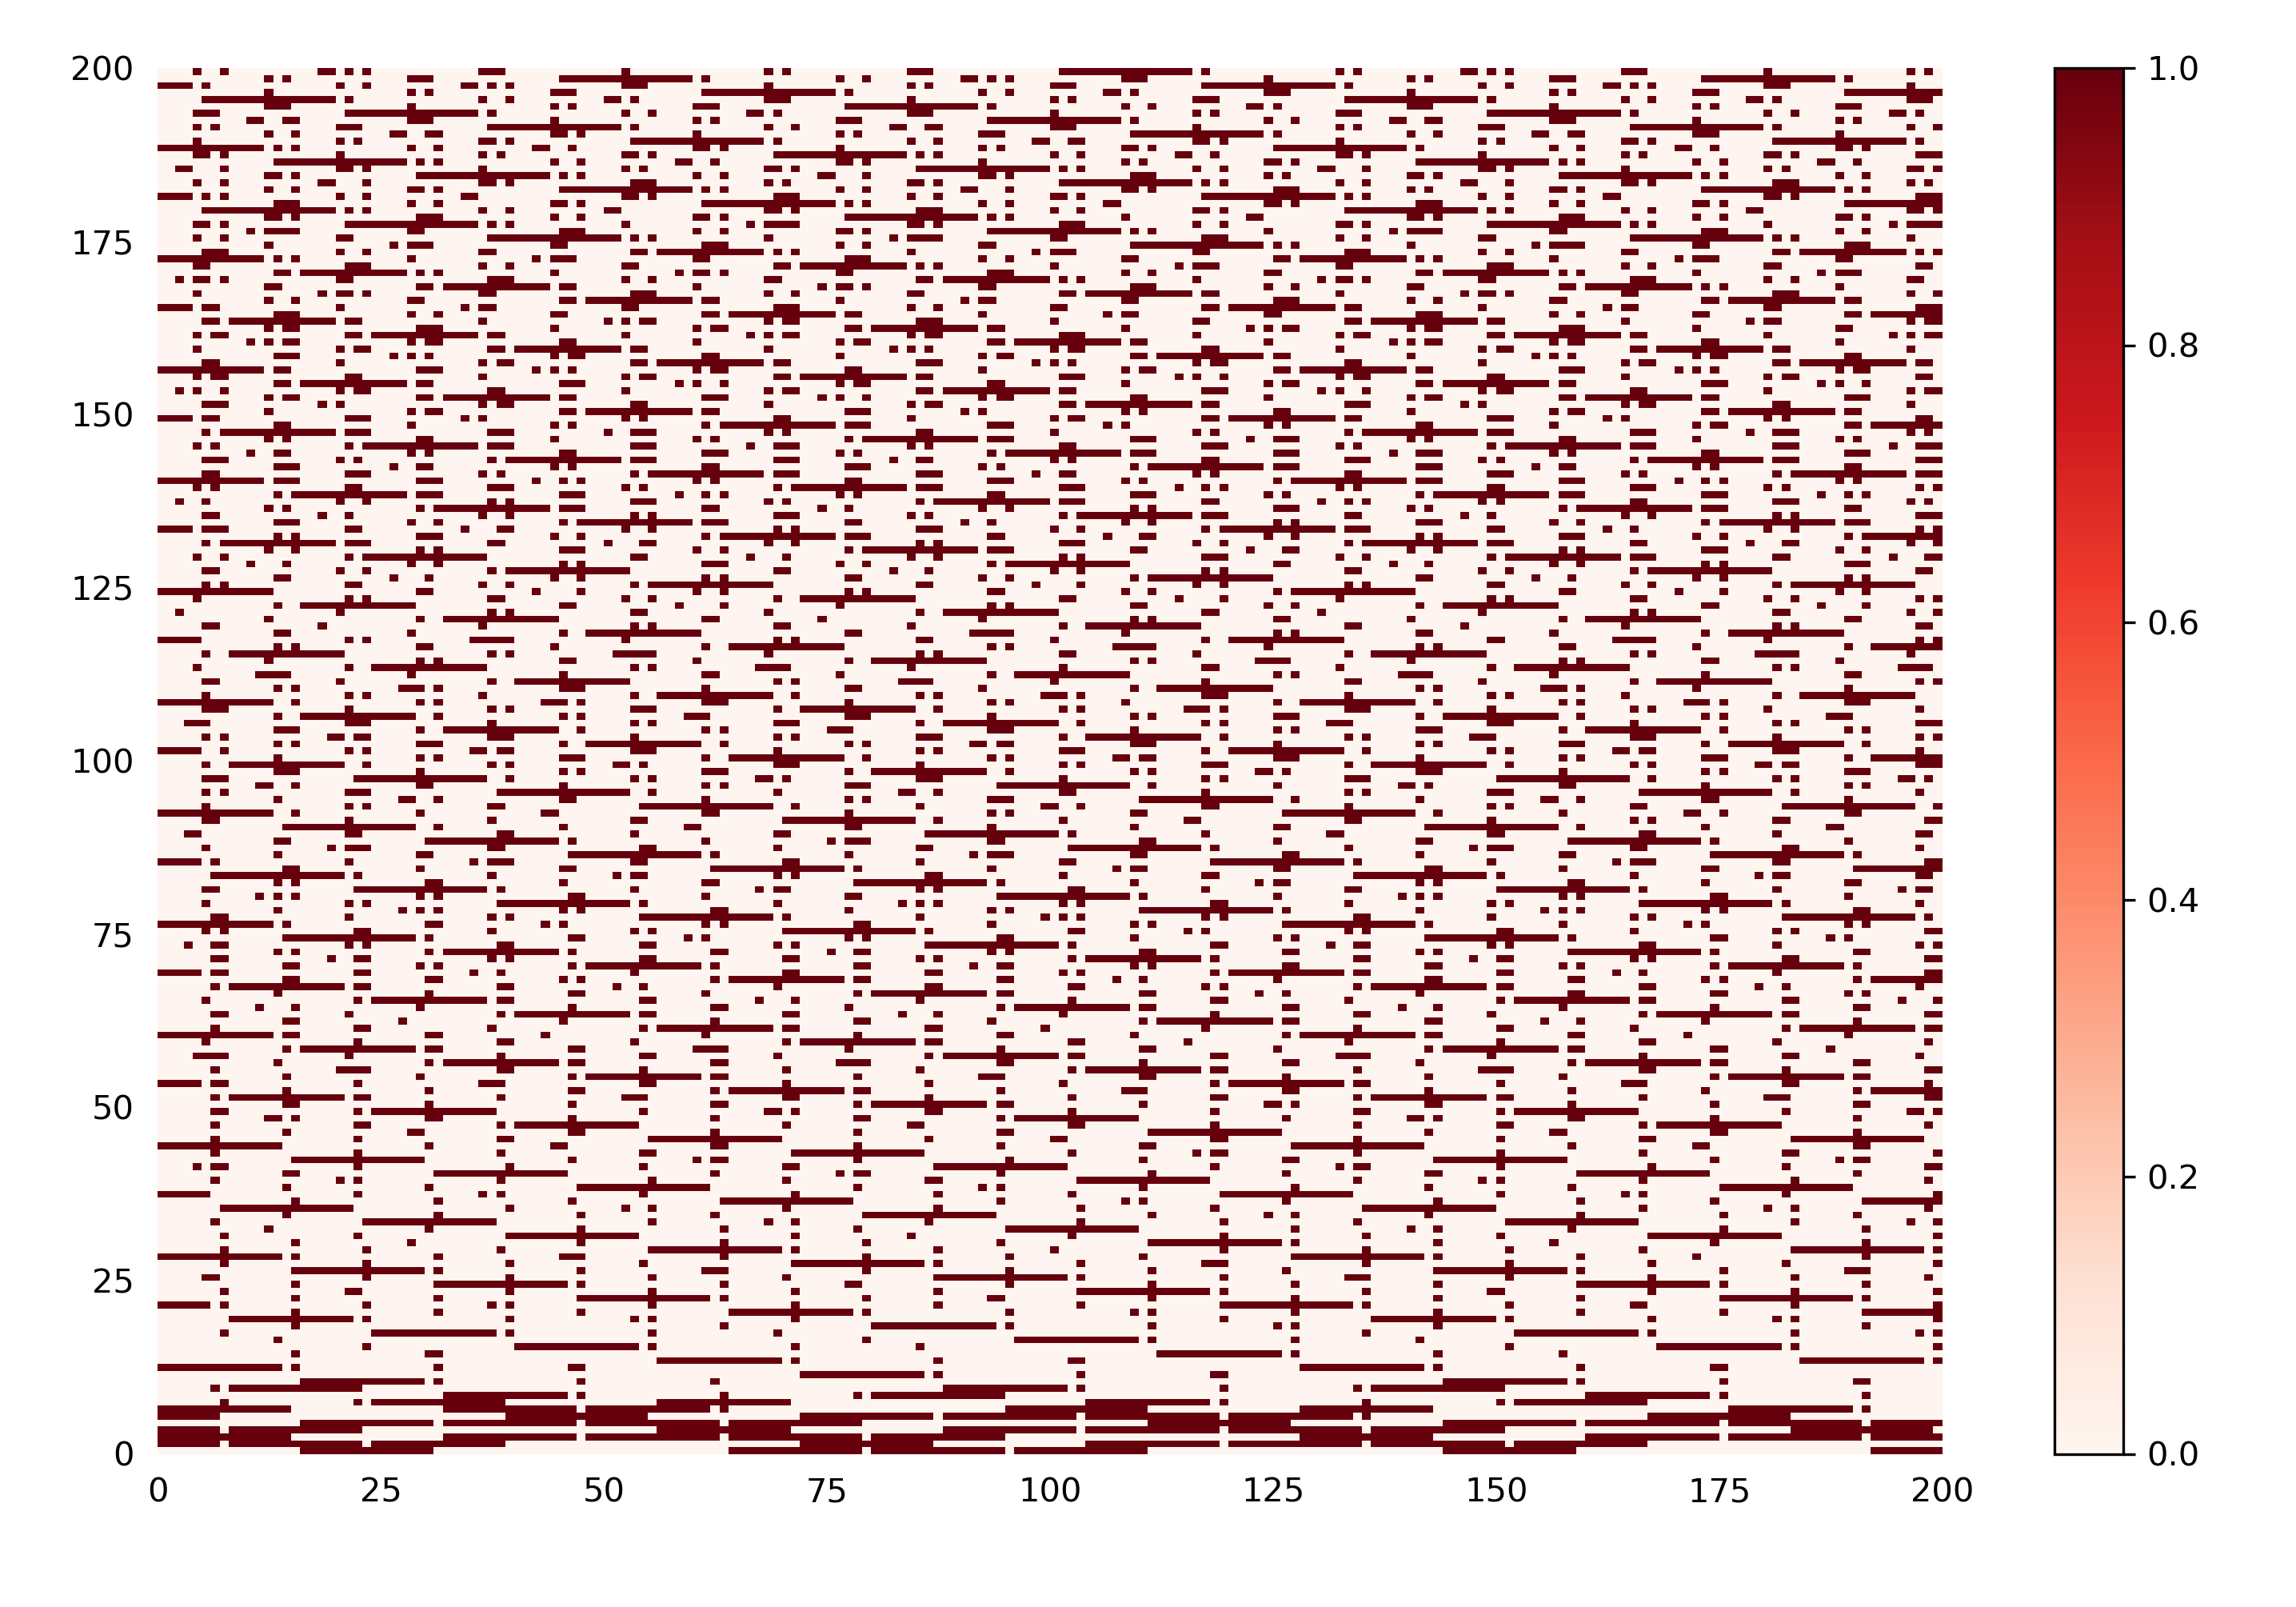
\includegraphics[width=0.85\textwidth]{img/discriminative_before}\\
    \caption{Visualization of the generator output as produced in the 9th discriminative training instance, before training. The first 40000 bits are presented as a 200 by 200 grid. The non-randomness of the output is obvious due to the visible patterns.}
    \label{figure:visualize_discriminative_before}
    \end{figure}
    
    \begin{figure}
    \centering
    \textbf{Output Sample, After Discriminative Training}
    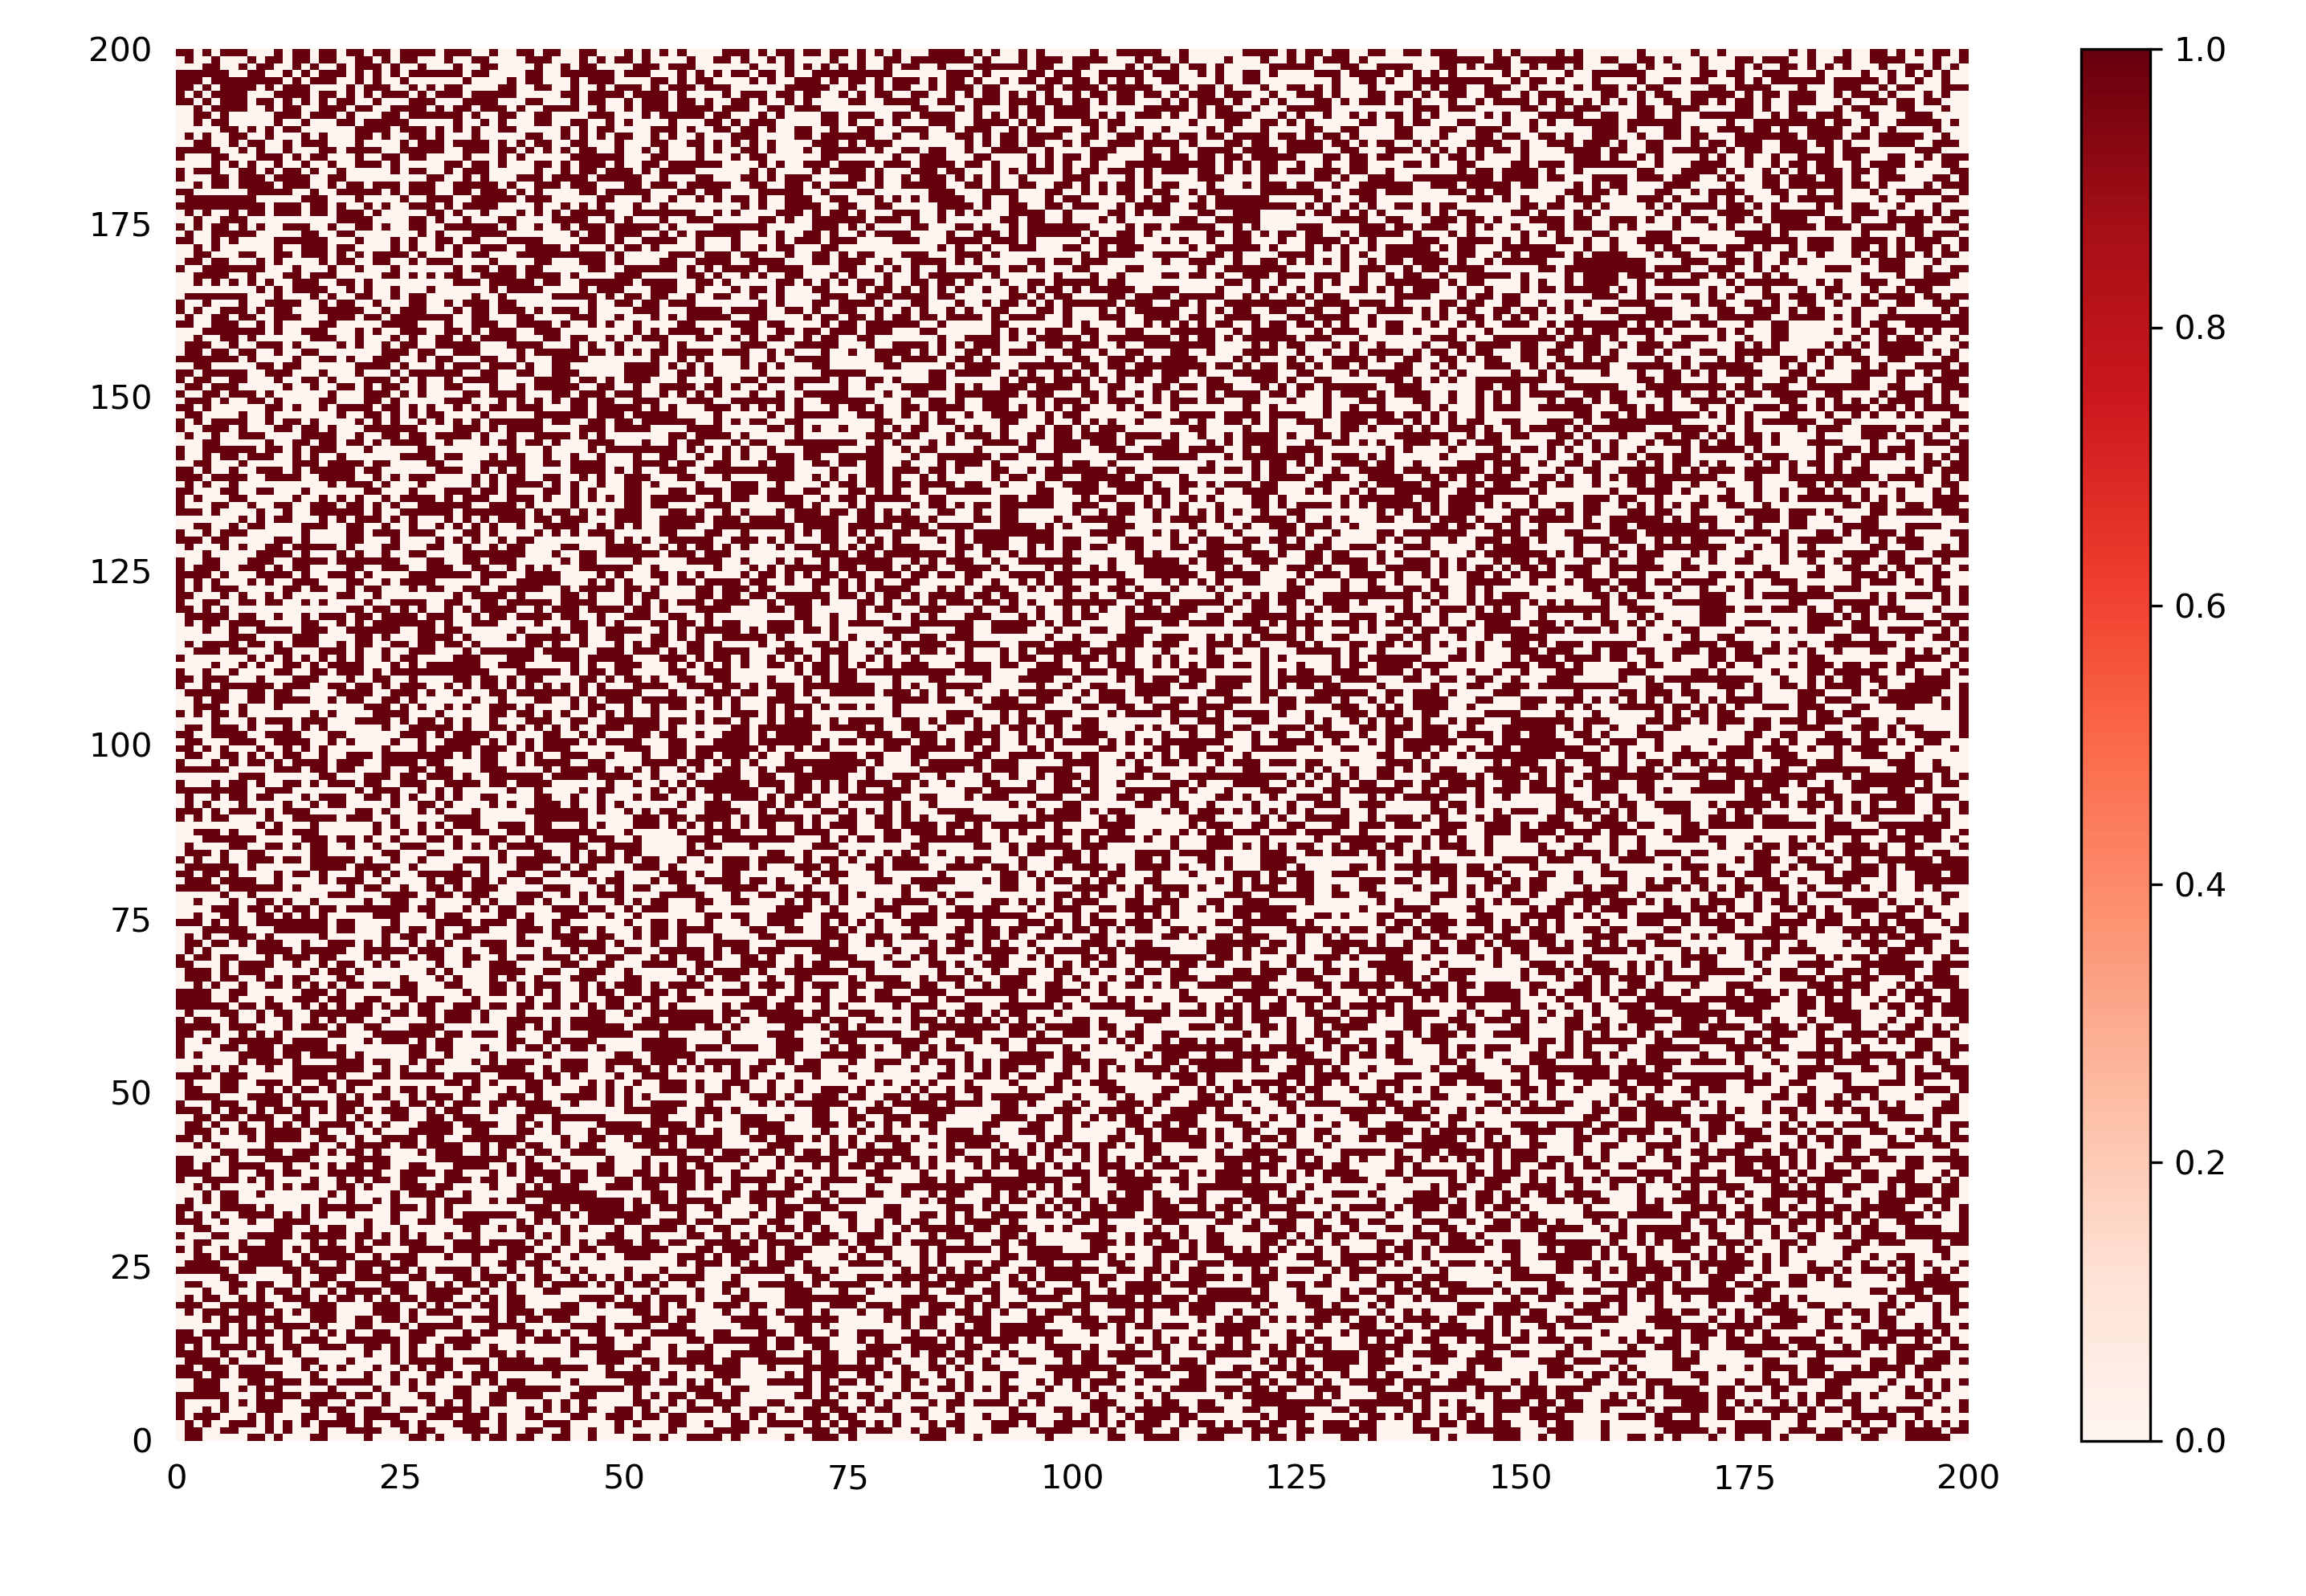
\includegraphics[width=0.85\textwidth]{img/discriminative_after}\\
    \caption{Visualization of the generator output as produced in the 9th discriminative training instance, after 200000 training iterations. The first 40000 bits are presented as a 200 by 200 grid. Clearly the generator neural network has learned to produce more randomness, as no patterns can reasonably be discerned by a human observer.}
    \label{figure:visualize_discriminative_after}
    \end{figure}
    
    \begin{figure}
    \centering
    \textbf{Output Sample, Before Predictive Training}
    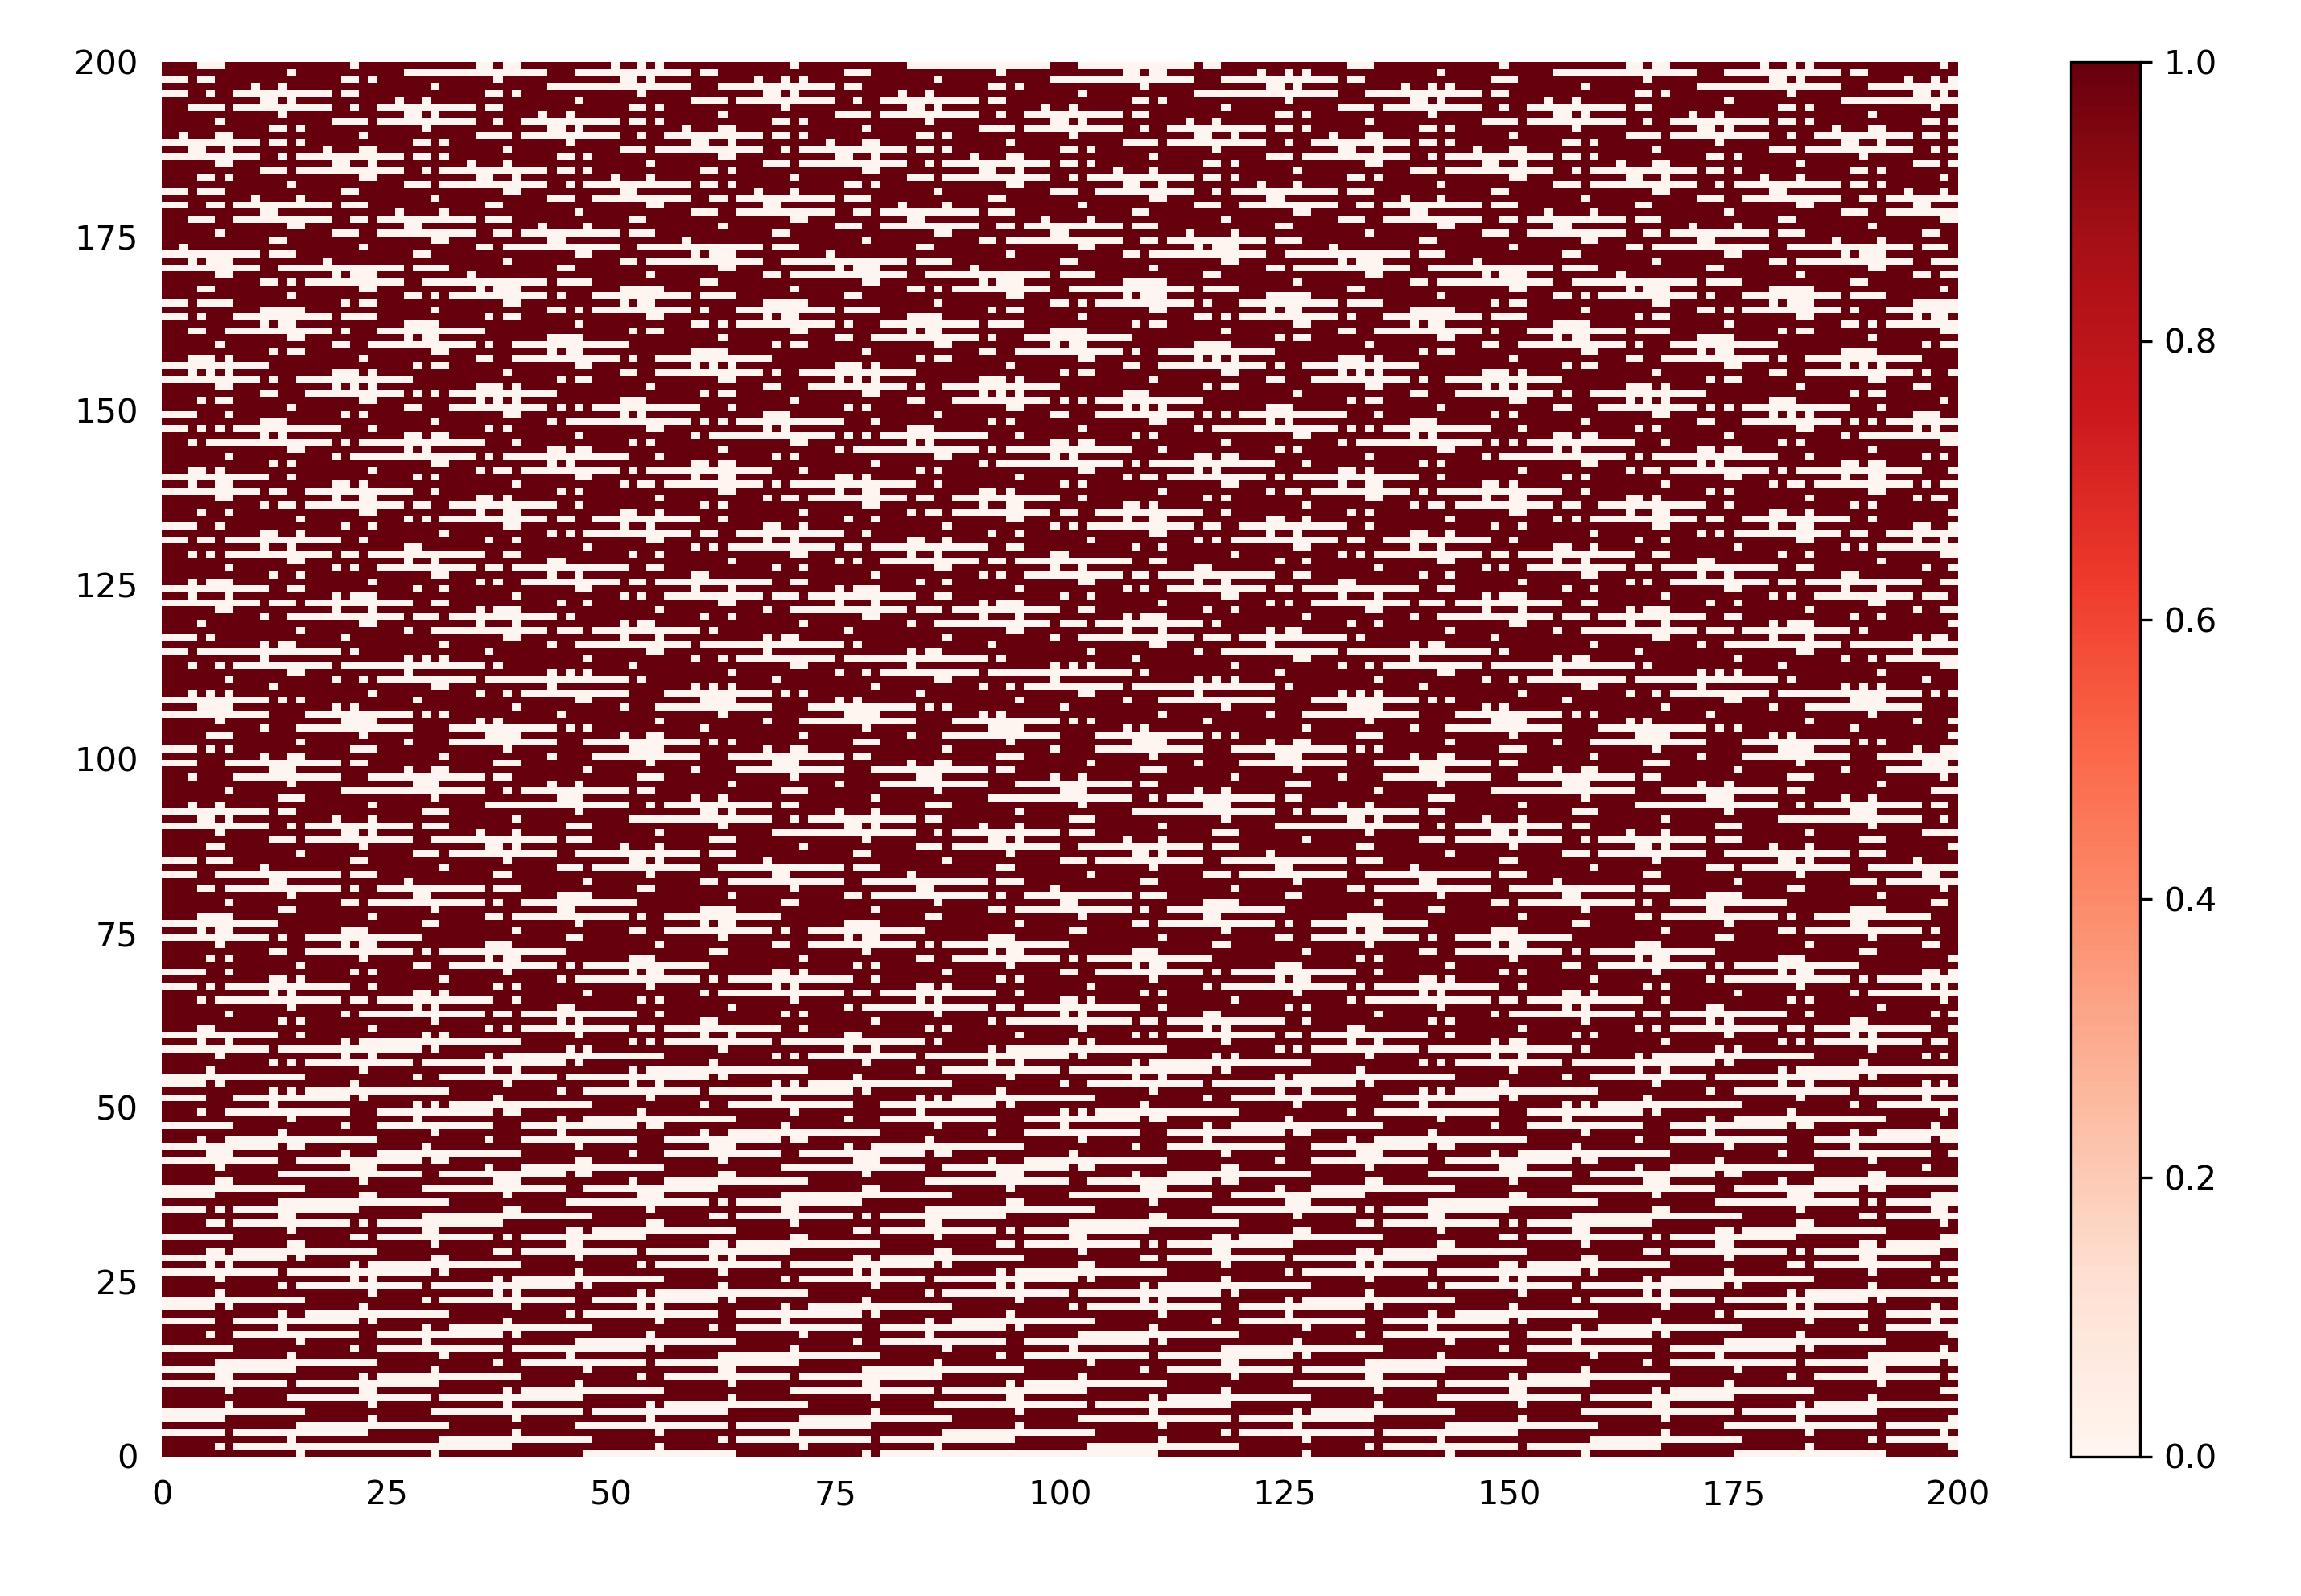
\includegraphics[width=0.85\textwidth]{img/predictive_before}\\
    \caption{Visualization of the generator output as produced in the 9th predictive training instance, before training. The first 40000 bits are presented as a 200 by 200 grid. The non-randomness of the output is obvious due to the visible patterns.}
    \label{figure:visualize_predictive_before}
    \end{figure}
    
    \begin{figure}
    \centering
    \textbf{Output Sample, After Predictive Training}
    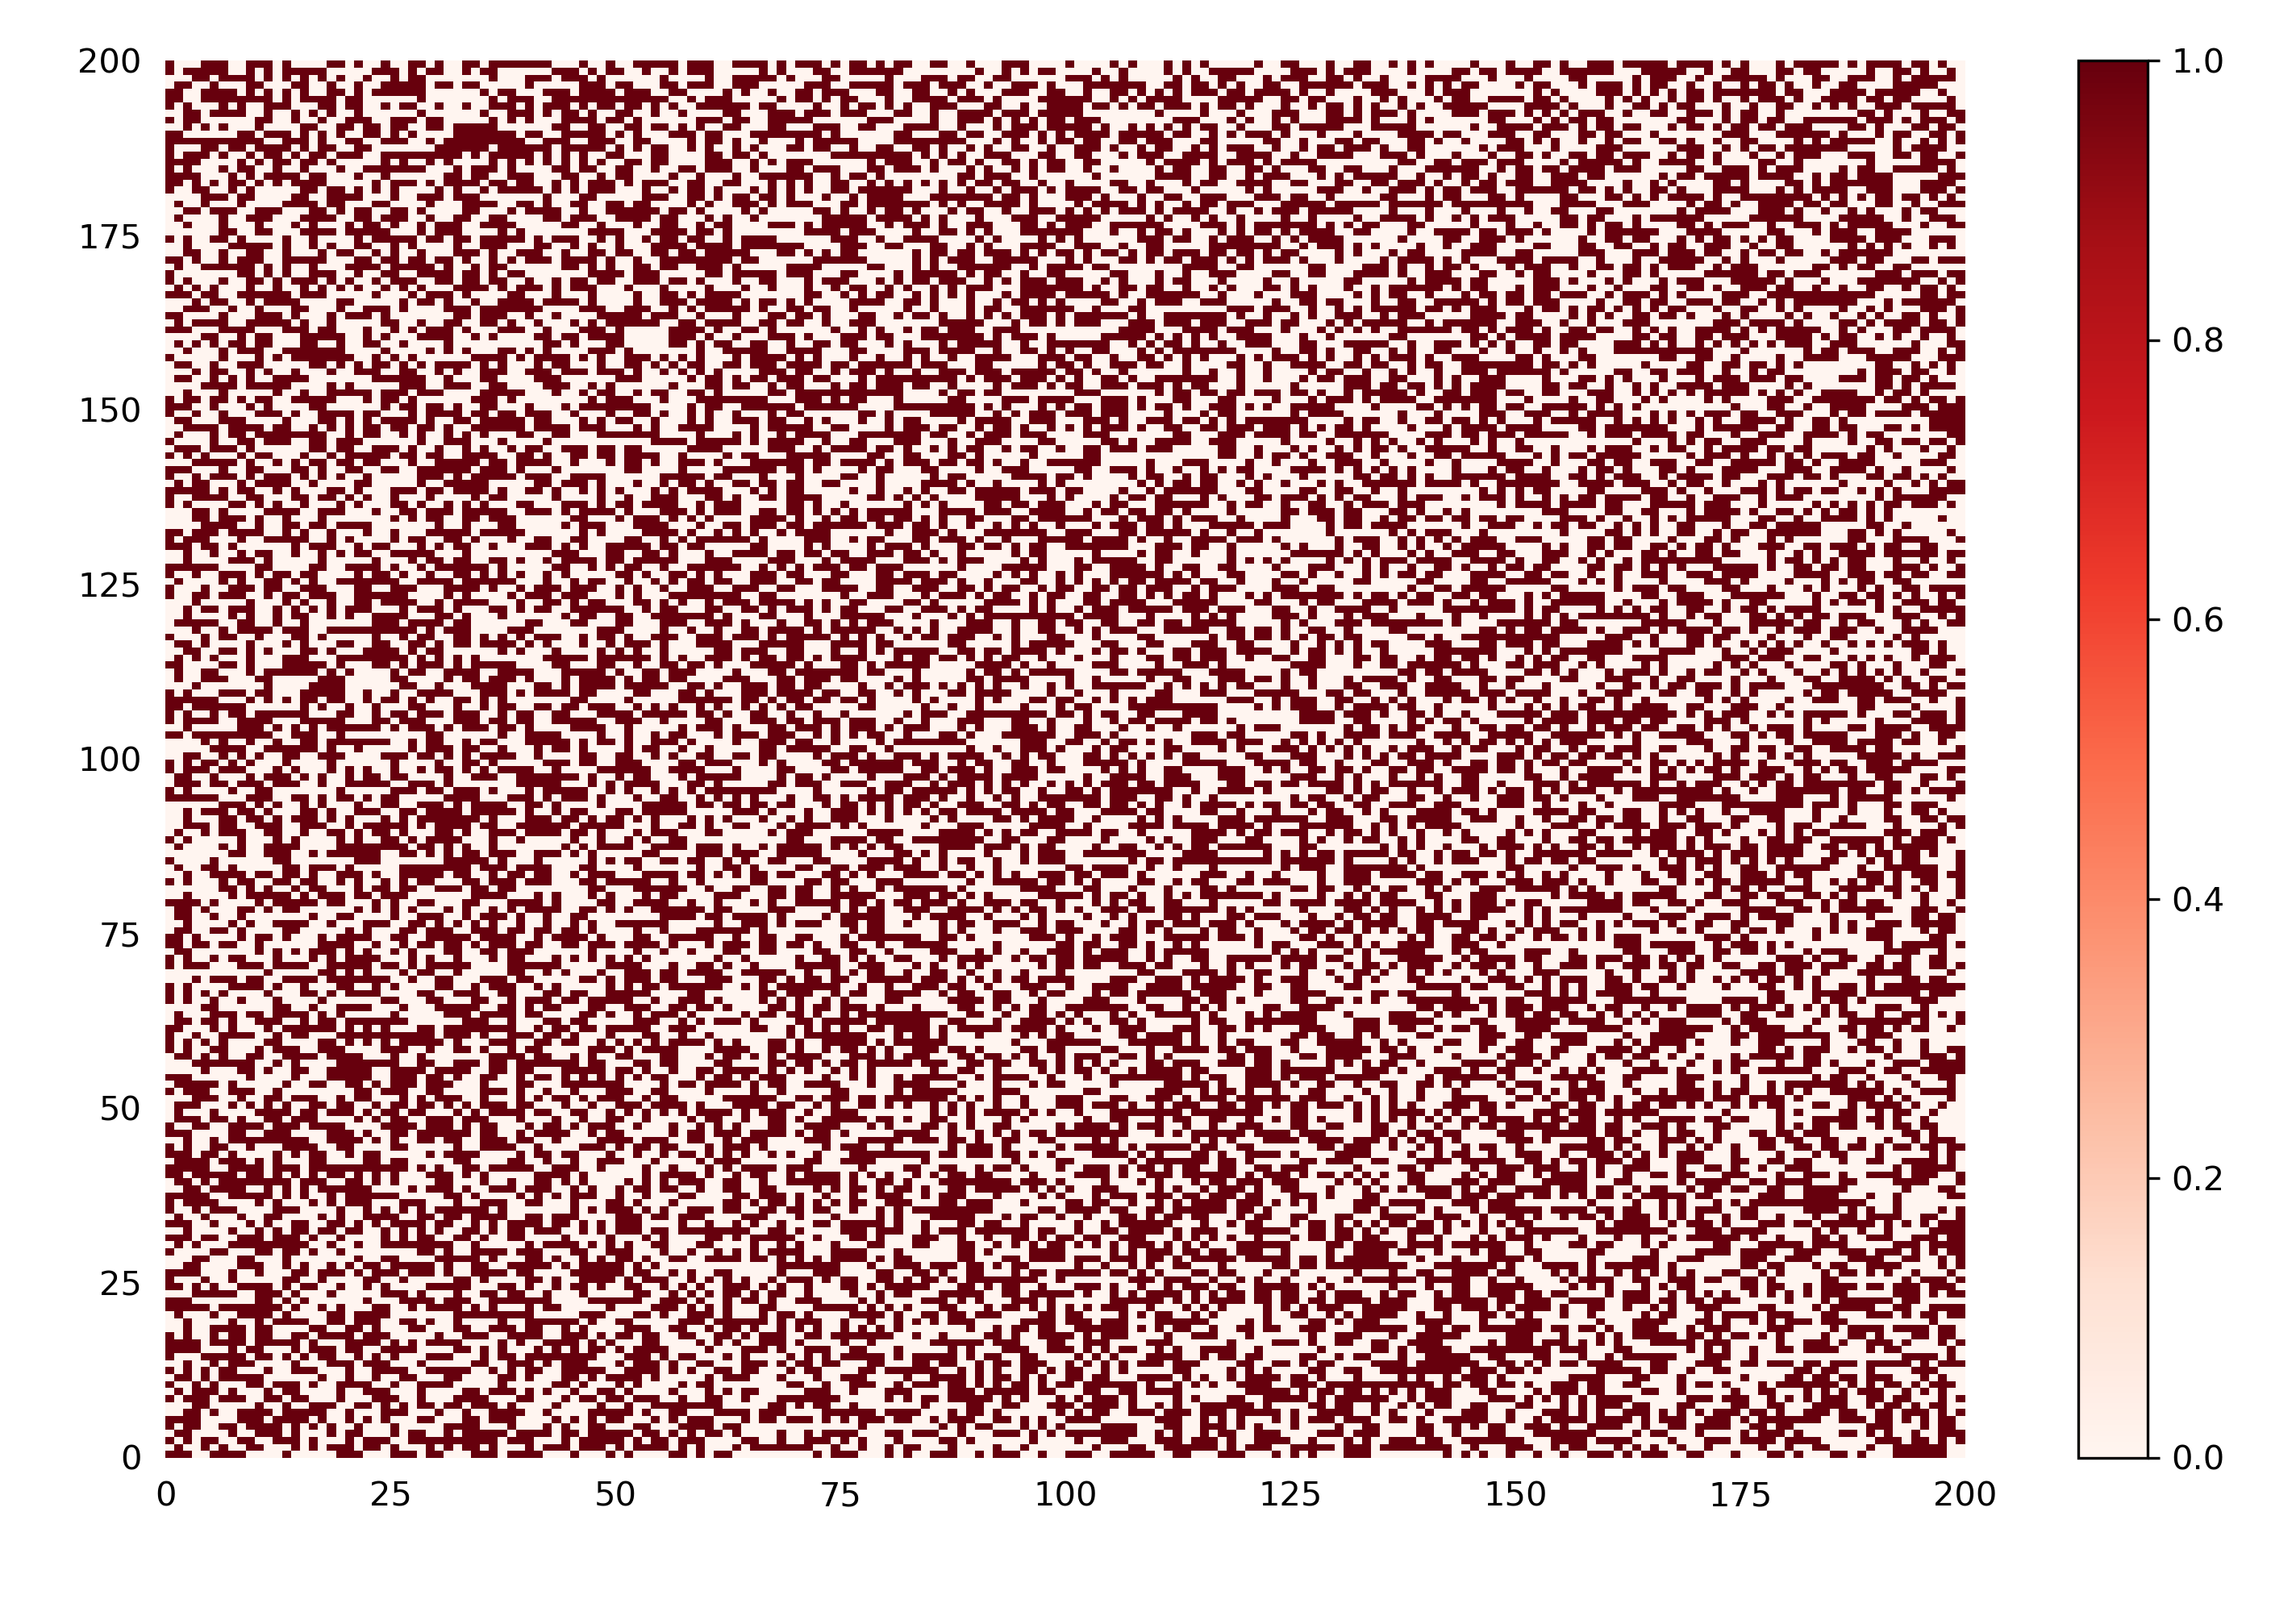
\includegraphics[width=0.85\textwidth]{img/predictive_after}\\
    \caption{Visualization of the generator output as produced in the 9th predictive training instance, after 200000 training iterations. The first 40000 bits are presented as a 200 by 200 grid. As with the discriminative training, no patterns can reasonably be discerned by a human observer; clearly the network has learned some notion of randomness.}
    \label{figure:visualize_predictive_after}
    \end{figure}



%----------------------------------------------------------
% CONCLUSION
%----------------------------------------------------------
\chapter{Conclusion}\label{chapter:conclusion}
Pseudo-random number generators, deterministic algorithms producing sequences of numbers which appear randomly sampled \cite[p. 7]{barker2007recommendation}, are used throughout the field of cryptography and are a fundamental element of many cryptographic systems such as encryption algorithms  \cite[p. 169]{menezes1996handbook} \cite[p. 1]{kelsey1998cryptanalytic}. As PRNGs are often a single point of failure for such systems, their design and analysis is an important field of investigation \cite[p. 2]{kelsey1998cryptanalytic} \cite{deng2017developments}. 

Machine learning, and in particular optimizeable parametric representations of non-linear functions called deep neural networks, has been tremendously successful in recent years \cite[p. 24-29]{russel2009artificial}. Despite this, the literature review carried out prior to this investigation suggests that little effort has gone into the application of machine learning methods to the implementation of PRNGs. Some attempts have been made with little success, and the papers are relatively obscure \cite{desai2011pseudo} \cite{desai2012pseudo} \cite{tirdad2010hopfield}.

The aim of this investigation was to determine whether a deep neural network can be trained to behave as a PRNG, and whether such a PRNG could be used in a cryptographic context. The scope of the investigation was limited to the statistical properties of a PRNG's output, and did not include cryptanalysis of the implementation. This work relies on the assumption that a neural network can represent a good pseudo-random function, and that discovering such a function by means of gradient descent is tractable. 

To accomplish the project aims, this project explored a novel approach, presenting two generative adversarial network (GAN) models designed to train a neural network to generate pseudo-random numbers. This avenue of investigation was motivated by the observation that the adversarial nature of GANs closely matches the roles of a PRNG and an adversary in a cryptographic context: the PRNG seeks to produce numbers that are unpredictable to the adversary, who attempts to predict future outputs. 

The design is based on three innovations. Firstly, the standard GAN approach is modified: one of the two approaches, termed the predictive approach, eliminates the need for a reference distribution, relying  solely on the interaction between the generator network and a convolutional predictor network trying to predict the generator's future outputs. This is contrasted with the classic discriminative approach, where a discriminator classifies input sequences as either belonging to the reference distribution, or as produced by the generator. The predictive approach is conceptually simpler and more efficient.

Furthermore, the deep neural network representing the generator uses a custom activation function at its output layer which computes a modulo operation on the network's outputs. This has a dramatic impact on the performance of the generator, presumably ``shuffling'' many of the patterns that may otherwise be discernible in the output.

Lastly, previous research in the field has used recurrent neural networks to model the statefulness of PRNGs, leading to complex systems that may be difficult to train. This work sidesteps these difficulties by implementing the generator as a simple stateless fully connected feed-forward network, where the state of the PRNG is modeled by additional non-random inputs to the model.

These design innovations resulted in a system that is elegant, conceptually simple, and robust. It is elegant in the sense that there is a close analogy between the structure of generative adversarial networks and the real-world security scenario involving a PRNG and a malicious agent. The system's simplicity and robustness are a result of the novel simplifications to the GAN architecture as well as the simple architecture of their constituent neural networks (in particular the generator).

This report has demonstrated that a generative adversarial network with the illustrated modifications can train the generator in such a manner as to produce pseudo-random number sequences with good statistical properties. In every experiment, the generator's performance on the NIST test suite improved from passing no tests to passing the majority of tests. At best, the generator could pass around 99\% of test instances, and around 98\% of unique tests. This metric alone does not justify use of the model in a cryptographic context, where a thorough cryptanalysis of the generator would be required, in addition to failing none of NIST's statistical tests.

As far as the author is aware, this novel research has matched, though not surpassed, the current state of the art in the generation of pseudo-random numbers using neural networks. Crucially, it has done so with a system that is much simpler and more robust than previous attempts, which have often been complicated even by their own authors' admission. Thanks to its simplicity, the approach considered in this work is easy to understand and modify. A number of obvious improvements to the system could be made, possibly producing even better results and warranting futher investigation.




%----------------------------------------------------------
% FURTHER INVESTIGATION
%----------------------------------------------------------
\chapter{Further Investigation}
The strong PRNG performance of the proposed generative adversarial networks, combined with the simplicity and robustness of the approach, suggest that the topic merits further investigation.
Additional tests beyond the scope of this investigation were carried out to determine whether increasing the generator's size or input dimensionality would improve performance. However, the analysis of these experiments could not be included in this report. A number of suggestions for further research include:

\textbf{Architectural Cross-Validation}. The architecture of the neural networks was chosen by intuition as well as by trial-and-error. Systematic cross-validation of different architectures could improve performance. Especially the network structure, the input and output dimensions, the loss functions, and the gradient descent variant almost certainly have room for improvement.

\textbf{Hyperparameter Optimization}. The models' hyperparameters were also chosen by trial-and-error. Systematic hyperparameter search to fine-tune the model could improve performance. In particular, important hyperparameters such as learning rate and mini-batch size should be optimized \cite[Neural Networks Part 3: Learning and Ealuation]{karpathy2017cs231n}.

\textbf{Recurrent Neural Networks}. The use of recurrent networks may add further capabilities to the networks \cite[chap. 10]{goodfellow2016deep}.

\textbf{Cryptanalysis}. Formal cryptanalysis of the implementation should be performed to determine whether a GAN-based PRNG can truly be cryptographically secure \cite[Abstract]{rukhin2001statistical}. 

\textbf{Potential Applications}. Potential applications of the system should also be considered. This could include existing public-key encryption algorithms that make use of random numbers, such as RSA. It could also include entirely new algorithms. For example, a hypothetical symmetric-key encryption/decryption algorithm could entail two communicating entities using synchronized neural network CSPRNGs. The two networks could independently and secretly generate the same encryption/decryption key for each message being transmitted. Initial synchronization could be performed by transmitting a truly random seed and a truly random sequence offset, using a key exchange protocol like Diffie-Hellman key exchange \cite[p. 174-177]{anderson2010security}.






%--------------------------------------------------
% BIBLIOGRAPHY
%--------------------------------------------------
\bibliographystyle{plain}
\bibliography{references.bib}


%----------------------------------------------------------
% APPENDICES
%----------------------------------------------------------
\appendix
\chapter{Glossary}



\chapter{Statistical Test Result Sample}\label{appendix:sample}
The outputs of the NIST test suite are extensive and cannot be fully reproduced in this appendix. One output report, produced for the 9th training instance of the predictive approach, is provided as an example.

\begin{minted}[fontsize=\footnotesize]{html}
------------------------------------------------------------------------------
RESULTS FOR THE UNIFORMITY OF P-VALUES AND THE PROPORTION OF PASSING SEQUENCES
------------------------------------------------------------------------------
   generator is <1_janice_dieharder.txt>
------------------------------------------------------------------------------
 C1  C2  C3  C4  C5  C6  C7  C8  C9 C10  P-VALUE  PROPORTION  STATISTICAL TEST
------------------------------------------------------------------------------
  1   0   0   0   0   1   2   2   1   3  0.350485     10/10      Frequency
  2   2   0   1   0   0   0   2   2   1  0.534146      9/10      BlockFrequency
  1   0   0   0   0   2   0   1   2   4  0.066882     10/10      CumulativeSums
  1   0   0   0   0   2   0   1   0   6  0.000199     10/10      CumulativeSums
  0   0   0   0   3   0   2   2   2   1  0.213309     10/10      Runs
  1   0   1   3   0   1   2   0   1   1  0.534146     10/10      LongestRun
  7   0   1   1   1   0   0   0   0   0  0.000003 *    4/10   *  Rank
 10   0   0   0   0   0   0   0   0   0  0.000000 *    0/10   *  FFT
  0   0   0   2   0   1   2   2   1   2  0.534146     10/10      NonOverlappingTemplate
  1   1   0   2   1   0   0   1   2   2  0.739918     10/10      NonOverlappingTemplate
  1   2   2   0   1   1   0   1   1   1  0.911413     10/10      NonOverlappingTemplate
  0   1   1   2   0   1   2   2   1   0  0.739918     10/10      NonOverlappingTemplate
  0   1   0   1   2   0   2   1   0   3  0.350485     10/10      NonOverlappingTemplate
  1   2   0   0   2   1   0   1   2   1  0.739918     10/10      NonOverlappingTemplate
  0   1   1   0   0   0   2   3   1   2  0.350485     10/10      NonOverlappingTemplate
  2   1   3   0   0   0   1   0   1   2  0.350485     10/10      NonOverlappingTemplate
  0   0   0   2   0   3   0   3   0   2  0.066882     10/10      NonOverlappingTemplate
  2   0   1   1   2   0   1   1   1   1  0.911413     10/10      NonOverlappingTemplate
  0   0   2   1   1   1   1   1   2   1  0.911413     10/10      NonOverlappingTemplate
  2   2   2   0   1   1   0   1   1   0  0.739918      9/10      NonOverlappingTemplate
  1   0   0   1   3   1   1   1   0   2  0.534146     10/10      NonOverlappingTemplate
  0   1   0   0   1   0   0   2   4   2  0.066882     10/10      NonOverlappingTemplate
  1   0   2   2   0   0   2   0   1   2  0.534146     10/10      NonOverlappingTemplate
  0   2   1   1   1   0   1   2   1   1  0.911413     10/10      NonOverlappingTemplate
  0   0   1   2   0   3   1   1   1   1  0.534146     10/10      NonOverlappingTemplate
  3   0   2   2   0   0   1   2   0   0  0.213309     10/10      NonOverlappingTemplate
  1   2   1   1   1   1   1   1   1   0  0.991468     10/10      NonOverlappingTemplate
  0   2   1   1   0   2   2   1   0   1  0.739918     10/10      NonOverlappingTemplate
  0   1   3   1   1   0   0   2   2   0  0.350485     10/10      NonOverlappingTemplate
  1   1   0   1   1   2   1   1   0   2  0.911413     10/10      NonOverlappingTemplate
  2   2   0   1   2   0   2   1   0   0  0.534146      9/10      NonOverlappingTemplate
  1   2   2   0   3   0   1   1   0   0  0.350485     10/10      NonOverlappingTemplate
  1   0   0   0   0   0   1   1   3   4  0.035174     10/10      NonOverlappingTemplate
  1   2   0   1   0   1   1   0   1   3  0.534146     10/10      NonOverlappingTemplate
  0   2   3   2   0   0   0   0   1   2  0.213309     10/10      NonOverlappingTemplate
  3   2   1   0   2   1   0   0   1   0  0.350485     10/10      NonOverlappingTemplate
  1   0   1   2   1   1   0   2   2   0  0.739918     10/10      NonOverlappingTemplate
  0   0   2   2   0   2   0   1   2   1  0.534146     10/10      NonOverlappingTemplate
  0   0   1   0   1   2   3   2   1   0  0.350485     10/10      NonOverlappingTemplate
  1   0   1   1   1   0   1   2   1   2  0.911413     10/10      NonOverlappingTemplate
  0   5   0   1   0   0   1   1   0   2  0.008879     10/10      NonOverlappingTemplate
  1   1   0   1   3   0   0   0   0   4  0.035174     10/10      NonOverlappingTemplate
  2   2   1   0   0   2   0   1   1   1  0.739918     10/10      NonOverlappingTemplate
  1   2   1   0   1   2   1   0   2   0  0.739918     10/10      NonOverlappingTemplate
  1   4   1   0   0   1   3   0   0   0  0.035174      9/10      NonOverlappingTemplate
  0   0   0   0   3   1   1   2   2   1  0.350485     10/10      NonOverlappingTemplate
  0   2   1   0   4   2   1   0   0   0  0.066882     10/10      NonOverlappingTemplate
  1   3   1   1   0   1   0   2   0   1  0.534146     10/10      NonOverlappingTemplate
  3   0   0   3   1   0   2   1   0   0  0.122325     10/10      NonOverlappingTemplate
  3   3   1   0   1   0   0   1   0   1  0.213309     10/10      NonOverlappingTemplate
  2   0   1   2   3   0   0   0   0   2  0.213309      9/10      NonOverlappingTemplate
  2   1   0   0   2   1   1   1   1   1  0.911413     10/10      NonOverlappingTemplate
  1   0   0   0   3   2   1   2   1   0  0.350485     10/10      NonOverlappingTemplate
  0   0   0   1   3   1   0   3   0   2  0.122325     10/10      NonOverlappingTemplate
  0   1   2   2   0   2   1   0   1   1  0.739918     10/10      NonOverlappingTemplate
  0   0   1   3   2   2   0   1   0   1  0.350485     10/10      NonOverlappingTemplate
  2   2   2   1   0   1   1   0   0   1  0.739918      9/10      NonOverlappingTemplate
  0   1   1   0   0   2   0   2   2   2  0.534146     10/10      NonOverlappingTemplate
  1   1   1   0   1   1   2   1   1   1  0.991468      9/10      NonOverlappingTemplate
  1   0   1   0   3   1   0   2   1   1  0.534146     10/10      NonOverlappingTemplate
  2   1   2   0   2   0   2   0   0   1  0.534146      9/10      NonOverlappingTemplate
  0   1   0   1   1   0   2   0   3   2  0.350485     10/10      NonOverlappingTemplate
  0   0   2   2   3   1   0   0   1   1  0.350485     10/10      NonOverlappingTemplate
  0   0   2   1   0   2   1   2   1   1  0.739918     10/10      NonOverlappingTemplate
  2   1   3   0   0   1   0   1   2   0  0.350485     10/10      NonOverlappingTemplate
  2   1   3   1   1   2   0   0   0   0  0.350485     10/10      NonOverlappingTemplate
  1   1   2   1   0   0   0   2   3   0  0.350485     10/10      NonOverlappingTemplate
  0   1   0   2   2   1   1   2   1   0  0.739918     10/10      NonOverlappingTemplate
  0   1   0   1   0   1   2   1   4   0  0.122325     10/10      NonOverlappingTemplate
  1   1   2   3   0   1   1   0   1   0  0.534146     10/10      NonOverlappingTemplate
  0   1   1   0   1   1   0   3   0   3  0.213309     10/10      NonOverlappingTemplate
  0   0   1   1   2   0   0   3   1   2  0.350485     10/10      NonOverlappingTemplate
  0   1   0   2   2   2   1   0   1   1  0.739918     10/10      NonOverlappingTemplate
  1   1   0   0   0   1   3   2   1   1  0.534146     10/10      NonOverlappingTemplate
  0   1   1   0   1   2   3   0   1   1  0.534146     10/10      NonOverlappingTemplate
  0   1   1   1   1   0   1   3   1   1  0.739918     10/10      NonOverlappingTemplate
  0   1   2   4   1   0   0   1   1   0  0.122325     10/10      NonOverlappingTemplate
  1   0   1   1   1   2   1   2   1   0  0.911413     10/10      NonOverlappingTemplate
  0   1   1   0   2   1   0   2   2   1  0.739918     10/10      NonOverlappingTemplate
  1   0   1   4   1   1   1   0   1   0  0.213309     10/10      NonOverlappingTemplate
  3   1   2   2   0   0   0   0   1   1  0.350485     10/10      NonOverlappingTemplate
  0   1   1   1   1   1   0   2   0   3  0.534146     10/10      NonOverlappingTemplate
  0   0   0   2   0   1   2   2   1   2  0.534146     10/10      NonOverlappingTemplate
  0   3   1   1   1   1   1   1   0   1  0.739918     10/10      NonOverlappingTemplate
  0   1   1   0   1   2   2   0   2   1  0.739918     10/10      NonOverlappingTemplate
  1   0   4   0   0   0   0   2   1   2  0.066882      9/10      NonOverlappingTemplate
  2   0   1   0   0   3   2   1   0   1  0.350485      9/10      NonOverlappingTemplate
  1   2   1   2   0   3   0   1   0   0  0.350485     10/10      NonOverlappingTemplate
  1   1   0   1   1   3   2   0   1   0  0.534146     10/10      NonOverlappingTemplate
  1   1   0   0   1   2   2   1   2   0  0.739918     10/10      NonOverlappingTemplate
  0   1   1   1   0   0   3   0   2   2  0.350485     10/10      NonOverlappingTemplate
  1   0   1   1   2   2   0   2   0   1  0.739918     10/10      NonOverlappingTemplate
  1   1   1   1   1   0   1   2   1   1  0.991468     10/10      NonOverlappingTemplate
  0   0   0   0   0   2   1   3   1   3  0.122325     10/10      NonOverlappingTemplate
  0   1   0   1   2   1   2   1   2   0  0.739918     10/10      NonOverlappingTemplate
  0   0   0   2   1   0   2   1   1   3  0.350485     10/10      NonOverlappingTemplate
  0   0   0   2   1   4   1   0   0   2  0.066882     10/10      NonOverlappingTemplate
  4   1   0   1   1   0   0   0   2   1  0.122325      9/10      NonOverlappingTemplate
  0   0   3   0   0   3   0   0   3   1  0.035174     10/10      NonOverlappingTemplate
  1   0   0   1   2   1   0   3   1   1  0.534146     10/10      NonOverlappingTemplate
  1   0   0   2   0   3   0   1   2   1  0.350485     10/10      NonOverlappingTemplate
  1   0   3   0   0   1   2   2   0   1  0.350485     10/10      NonOverlappingTemplate
  1   1   0   2   0   3   1   2   0   0  0.350485     10/10      NonOverlappingTemplate
  2   2   0   1   0   0   0   2   1   2  0.534146     10/10      NonOverlappingTemplate
  0   0   1   2   2   3   1   0   1   0  0.350485     10/10      NonOverlappingTemplate
  1   0   1   1   1   1   1   2   2   0  0.911413     10/10      NonOverlappingTemplate
  1   1   1   0   2   0   1   1   0   3  0.534146     10/10      NonOverlappingTemplate
  0   1   2   2   0   0   1   1   2   1  0.739918     10/10      NonOverlappingTemplate
  0   0   0   2   0   1   1   4   0   2  0.066882     10/10      NonOverlappingTemplate
  0   1   1   2   2   1   0   1   1   1  0.911413     10/10      NonOverlappingTemplate
  1   0   1   0   1   1   0   2   1   3  0.534146     10/10      NonOverlappingTemplate
  3   1   1   1   0   2   0   1   0   1  0.534146      8/10      NonOverlappingTemplate
  1   1   0   0   1   2   4   0   1   0  0.122325     10/10      NonOverlappingTemplate
  1   0   0   2   0   1   1   1   3   1  0.534146     10/10      NonOverlappingTemplate
  0   1   1   3   1   0   1   1   2   0  0.534146     10/10      NonOverlappingTemplate
  2   1   0   3   0   2   0   0   1   1  0.350485     10/10      NonOverlappingTemplate
  1   0   1   1   1   0   2   1   2   1  0.911413     10/10      NonOverlappingTemplate
  1   0   0   1   0   0   2   0   3   3  0.122325     10/10      NonOverlappingTemplate
  0   0   0   1   0   2   1   0   3   3  0.122325     10/10      NonOverlappingTemplate
  1   1   0   0   2   1   1   0   2   2  0.739918     10/10      NonOverlappingTemplate
  2   0   0   0   0   1   3   1   0   3  0.122325     10/10      NonOverlappingTemplate
  1   1   1   0   3   2   1   0   0   1  0.534146      9/10      NonOverlappingTemplate
  0   2   1   2   1   1   0   1   0   2  0.739918     10/10      NonOverlappingTemplate
  4   0   1   2   0   0   0   2   1   0  0.066882      9/10      NonOverlappingTemplate
  1   3   0   0   2   3   1   0   0   0  0.122325     10/10      NonOverlappingTemplate
  0   2   1   1   1   0   2   0   2   1  0.739918     10/10      NonOverlappingTemplate
  0   3   1   0   2   0   0   2   2   0  0.213309     10/10      NonOverlappingTemplate
  1   2   1   0   0   1   2   1   1   1  0.911413     10/10      NonOverlappingTemplate
  0   0   4   1   2   2   0   1   0   0  0.066882     10/10      NonOverlappingTemplate
  2   1   0   2   0   1   0   1   1   2  0.739918     10/10      NonOverlappingTemplate
  1   2   1   0   0   1   0   2   0   3  0.350485     10/10      NonOverlappingTemplate
  1   0   0   1   1   1   0   0   2   4  0.122325     10/10      NonOverlappingTemplate
  0   1   1   2   1   1   1   1   1   1  0.991468     10/10      NonOverlappingTemplate
  1   1   6   1   0   0   0   0   1   0  0.000439     10/10      NonOverlappingTemplate
  0   0   1   1   0   0   2   0   2   4  0.066882     10/10      NonOverlappingTemplate
  2   1   0   0   2   0   0   3   1   1  0.350485     10/10      NonOverlappingTemplate
  1   0   0   1   4   1   2   1   0   0  0.122325     10/10      NonOverlappingTemplate
  0   1   0   2   1   0   3   1   1   1  0.534146     10/10      NonOverlappingTemplate
  1   2   0   0   0   1   0   3   0   3  0.122325      9/10      NonOverlappingTemplate
  2   2   0   2   0   1   1   1   0   1  0.739918     10/10      NonOverlappingTemplate
  1   1   0   0   1   0   2   1   2   2  0.739918     10/10      NonOverlappingTemplate
  0   0   0   3   2   1   2   1   0   1  0.350485     10/10      NonOverlappingTemplate
  2   2   1   0   3   1   0   0   0   1  0.350485     10/10      NonOverlappingTemplate
  0   1   1   0   1   2   1   2   2   0  0.739918     10/10      NonOverlappingTemplate
  4   2   0   0   0   2   1   0   0   1  0.066882     10/10      NonOverlappingTemplate
  0   0   1   0   0   3   0   2   2   2  0.213309     10/10      NonOverlappingTemplate
  3   3   1   0   0   0   0   1   2   0  0.122325     10/10      NonOverlappingTemplate
  2   0   0   0   2   1   2   1   2   0  0.534146     10/10      NonOverlappingTemplate
  0   1   0   1   1   1   2   2   0   2  0.739918     10/10      NonOverlappingTemplate
  1   0   3   1   0   1   1   1   2   0  0.534146      9/10      NonOverlappingTemplate
  0   4   0   1   2   0   1   1   1   0  0.122325     10/10      NonOverlappingTemplate
  0   1   2   0   0   1   2   1   0   3  0.350485     10/10      NonOverlappingTemplate
  0   1   0   0   2   0   2   1   1   3  0.350485     10/10      NonOverlappingTemplate
  0   1   0   0   1   3   1   1   2   1  0.534146     10/10      NonOverlappingTemplate
  1   0   0   2   0   2   2   1   1   1  0.739918     10/10      NonOverlappingTemplate
  0   1   1   1   1   1   0   2   0   3  0.534146     10/10      NonOverlappingTemplate
  6   0   2   0   0   1   0   1   0   0  0.000199      7/10   *  OverlappingTemplate
  2   1   2   0   0   1   0   1   1   2  0.739918     10/10      Universal
  0   0   2   0   1   0   1   0   1   5  0.008879     10/10      ApproximateEntropy
  1   1   1   1   1   1   0   1   2   0     ----       9/9       RandomExcursions
  2   1   0   3   0   1   0   0   0   2     ----       9/9       RandomExcursions
  1   0   0   3   1   0   1   2   1   0     ----       9/9       RandomExcursions
  3   1   0   0   0   1   0   3   0   1     ----       9/9       RandomExcursions
  1   1   0   3   1   1   1   0   0   1     ----       9/9       RandomExcursions
  0   0   2   0   2   1   3   0   0   1     ----       9/9       RandomExcursions
  0   0   0   1   0   2   1   1   2   2     ----       9/9       RandomExcursions
  1   1   0   4   0   0   0   2   1   0     ----       9/9       RandomExcursions
  0   1   0   1   1   1   3   0   0   2     ----       9/9       RandomExcursionsVariant
  0   0   0   3   0   2   1   2   0   1     ----       9/9       RandomExcursionsVariant
  0   0   2   0   3   0   1   1   1   1     ----       9/9       RandomExcursionsVariant
  0   0   1   2   2   1   1   0   1   1     ----       9/9       RandomExcursionsVariant
  0   0   1   1   3   1   2   1   0   0     ----       9/9       RandomExcursionsVariant
  0   0   1   3   0   2   0   1   1   1     ----       9/9       RandomExcursionsVariant
  0   0   2   0   0   2   2   1   2   0     ----       9/9       RandomExcursionsVariant
  0   1   1   1   0   0   1   1   2   2     ----       9/9       RandomExcursionsVariant
  1   1   0   0   2   1   0   0   4   0     ----       9/9       RandomExcursionsVariant
  0   1   1   0   0   1   3   2   0   1     ----       9/9       RandomExcursionsVariant
  0   1   1   2   0   2   0   1   2   0     ----       9/9       RandomExcursionsVariant
  0   1   1   1   1   1   2   1   0   1     ----       9/9       RandomExcursionsVariant
  0   0   3   1   0   1   1   1   0   2     ----       9/9       RandomExcursionsVariant
  0   2   0   0   1   1   1   1   3   0     ----       9/9       RandomExcursionsVariant
  1   0   1   0   1   1   0   2   2   1     ----       9/9       RandomExcursionsVariant
  1   0   1   0   2   0   3   1   0   1     ----       9/9       RandomExcursionsVariant
  0   0   3   0   0   0   3   1   1   1     ----       9/9       RandomExcursionsVariant
  0   0   1   0   1   1   2   3   0   1     ----       9/9       RandomExcursionsVariant
  0   1   1   0   0   1   0   1   1   5  0.017912     10/10      Serial
  1   0   0   0   0   0   0   1   3   5  0.002043     10/10      Serial
  1   1   2   1   0   1   0   2   0   2  0.739918     10/10      LinearComplexity


- - - - - - - - - - - - - - - - - - - - - - - - - - - - - - - - - - - - - - - - -
The minimum pass rate for each statistical test with the exception of the
random excursion (variant) test is approximately = 8 for a
sample size = 10 binary sequences.

The minimum pass rate for the random excursion (variant) test
is approximately = 8 for a sample size = 9 binary sequences.

For further guidelines construct a probability table using the MAPLE program
provided in the addendum section of the documentation.
- - - - - - - - - - - - - - - - - - - - - - - - - - - - - - - - - - - - - - - - -
\end{minted}


\chapter{Summary of Supporting Material}
This appendix section lists all the material that is available externally to this report, and provides instructions for how to access it.

The software, as well as the results of all performed statistical testing, are available in the supporting documentation submitted. Instructions for executing the software are in the readme submitted as part of the supporting documentation. Results are stored in the \mintinline{html}{results} directory. The raw generator outputs are not included in the supporting documentation, since the 5GB of data far exceeds the upload size limit. Instead, the raw output can be accessed at the following link on the author's OneDrive file storage:

https://1drv.ms/f/s!Ah1ayeYeFEuDiJVILSrGN5x\_iiKSsw

Should the link not work, the author can provide a new link upon request. The link does not allow editing. The link points to a directory tree structured as follows:

\begin{minted}[fontsize=\footnotesize]{html}   
> results
    > discriminative
        > 01
            > after
            > before
            > plots
            > sequences            
        > 02
            ...
        ...
    > predictive
        > 01
            > after
            > before
            > plots
            > sequences
        > 02
            ...
        ...
\end{minted}

The numbered folders indicate the experiment. For each experiment, the subdirectories contain the results of statistical testing using NIST from before and after training, the logged training loss values, and the actual output sequences (the sequences with names prefixed by a 0 are generated before training, while the ones prefixed by 1 are generated after training). The same directory structure in included in the supporting documentation submitted directly, with exception of the \mintinline{python}{sequences} subdirectories as these are too large.

\end{document}
